% Pruning results to date on WSD, Viewsphere and COCO: datasets, methods, then results per dataset.
% Tables are generated into tables/ by make_tables.py from tina's results/same_protocol CSVs; the prose is here.
\documentclass[10pt]{article}
\usepackage[margin=1.8cm]{geometry}
\usepackage[T1]{fontenc}
\usepackage{lmodern}
\usepackage{amsmath}
\usepackage{booktabs}
\usepackage{adjustbox}
\usepackage{graphicx}  % figures/ made by win_chart.py
\usepackage{float}  % [H]: keep each table with its section
\usepackage{caption}
\usepackage{enumitem}
\usepackage[hidelinks]{hyperref}

\captionsetup{font=small,labelfont=bf,textfont=bf,position=top,skip=4pt}  % caption = the table's title, above it
\newcommand{\tnote}[1]{\par\vspace{3pt}\begin{minipage}{\linewidth}\footnotesize #1\end{minipage}}  % notes under a table
\setlist{itemsep=1pt,topsep=3pt}
\setlength{\parskip}{3pt}
\newcommand{\tbl}[1]{\adjustbox{max width=\linewidth}{\input{tables/#1}}}

\title{\vspace{-1.5em}Pruning YOLO26 and YOLOv5 on WSD, Viewsphere and COCO: results to date\vspace{-0.5em}}
\author{Blake J.\ Gisclair}
\date{\today}

\begin{document}
\maketitle

\noindent\textbf{Summary.} Every model here starts from COCO-pretrained weights fine-tuned on its
dataset (Section~\ref{sec:data}); this replaces the earlier version, whose WSD models were trained from
scratch. Right after pruning, the PEEK persistence scores (field~H1, H0, H0+H1) are the best channel
criteria on every dataset and both architectures: a persistence score wins 78 of 80 one-shot settings,
and L2 is often no better than random (on Viewsphere~v2, worse). After a 20-epoch fine-tune the
criteria converge on WSD (within about 0.01 mAP50-95), but on Viewsphere, Viewsphere~v2 and COCO the
persistence scores stay ahead, by a margin that grows with pruning (about +0.04 over L2 at 50\%,
averaged over models). Which of the three persistence scores leads is mostly within seed noise. For
block replacement the ranking matters more than the score, and the best one differs by dataset: the
null ranking scored on H1 on WSD, the raw head ranking and the new L2 weight-norm baseline on
Viewsphere, the null ranking on COCO. Channel pruning cuts up to 28\% of GFLOPs but only 1--4\% of GPU
latency. YOLOv5 (Section~\ref{sec:v5}) shows the same picture, and Viewsphere~v2 (17 satellites,
Section~\ref{sec:vs2}) now behaves like v1, after a fix for the renders' black backgrounds.
Figures~\ref{fig:w-wsd}--\ref{fig:wins} count how often each channel criterion comes out best: one
figure per dataset, then all four together. A setting = model (YOLO26n/s, YOLOv5n/s) $\times$ pruning
ratio (10--50\%), 20 per dataset; the criterion with the highest mean mAP50-95 over seeds wins it (ties
count for each). A win is a highest mean, not necessarily a lead beyond the seed noise (the
$^\dagger$ in the tables).

\begin{figure}[H]
\centering
\caption{WSD: which channel-pruning criterion wins most often}
\label{fig:w-wsd}
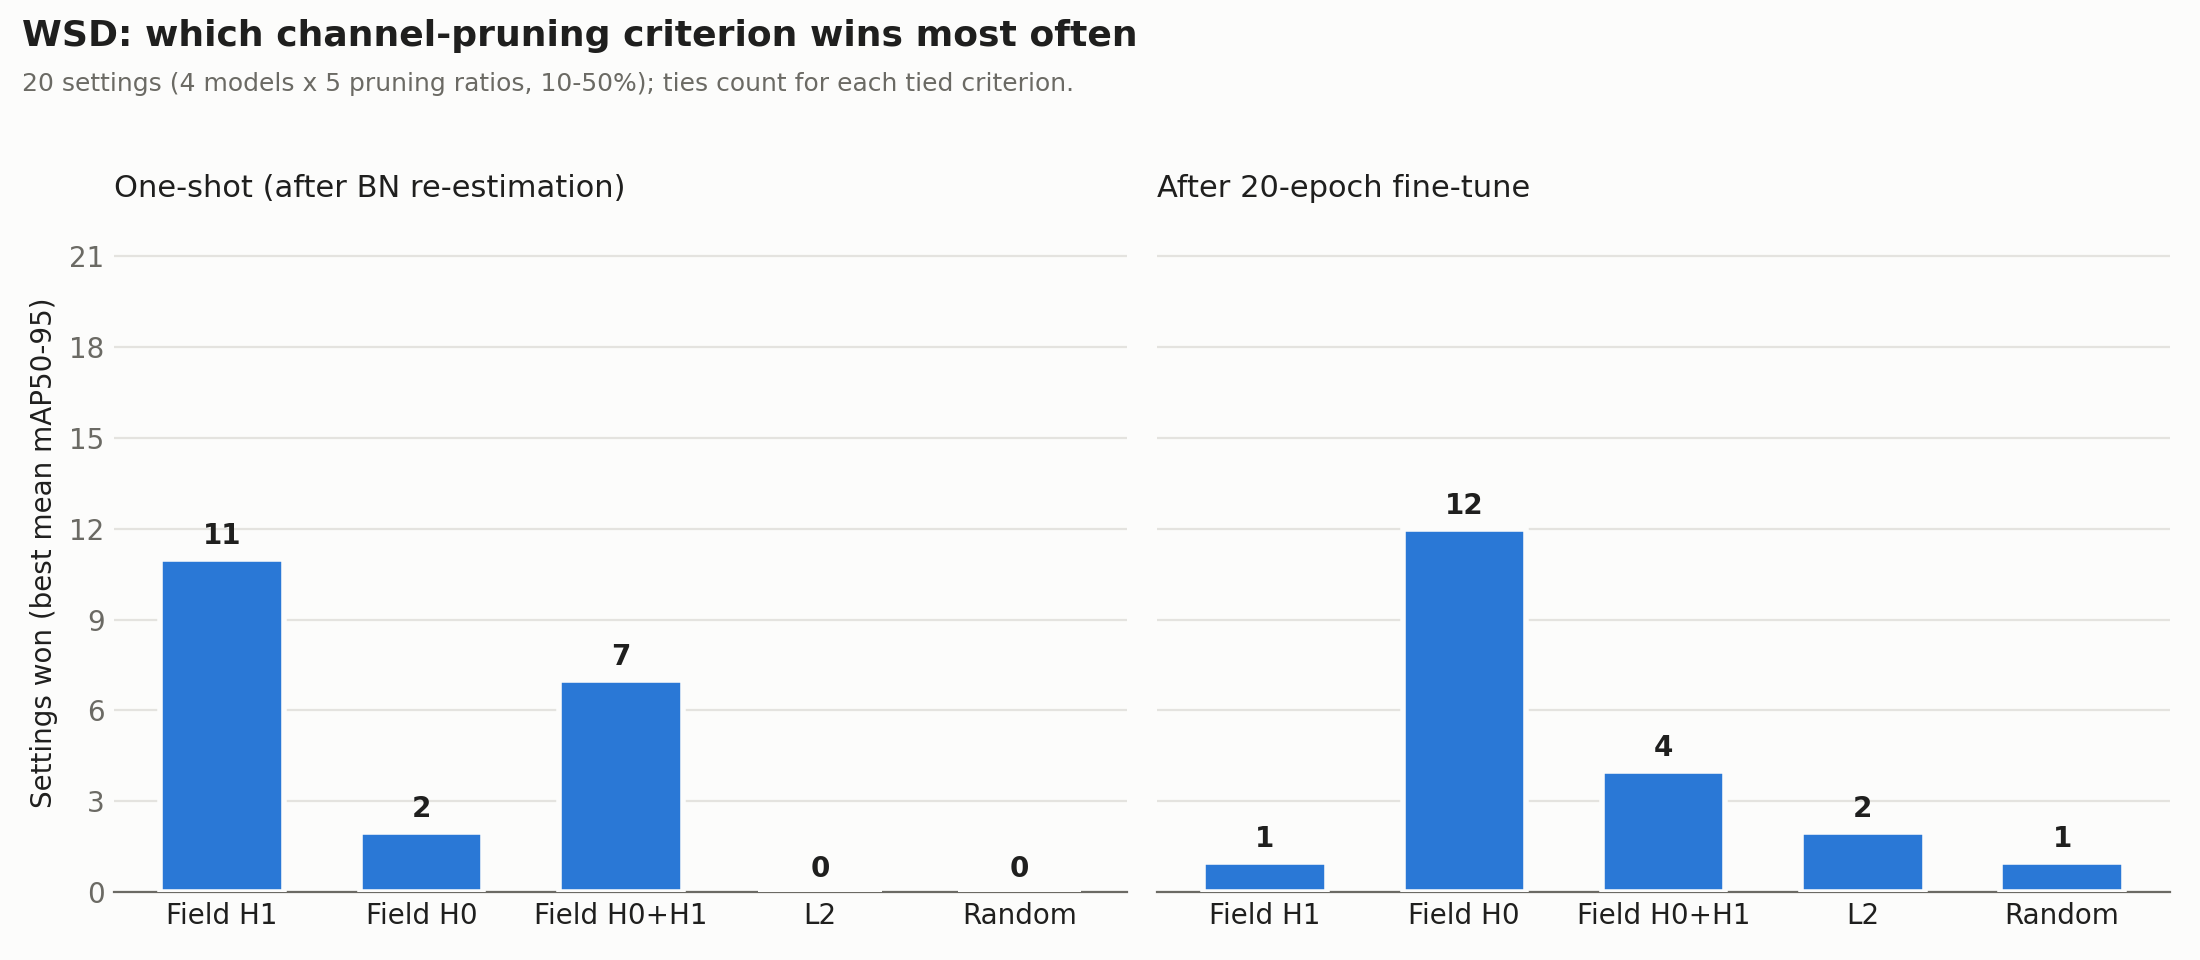
\includegraphics[width=\linewidth]{figures/criterion_wins_wsd.png}
\tnote{One-shot, a persistence score wins all 20 (field~H1 11, H0+H1 7, H0 2). After fine-tuning
field~H0 wins 12 of 20, but the criteria end within about 0.01 of each other (Table~\ref{tab:wsd}).}
\end{figure}

\begin{figure}[H]
\centering
\caption{Viewsphere: which channel-pruning criterion wins most often}
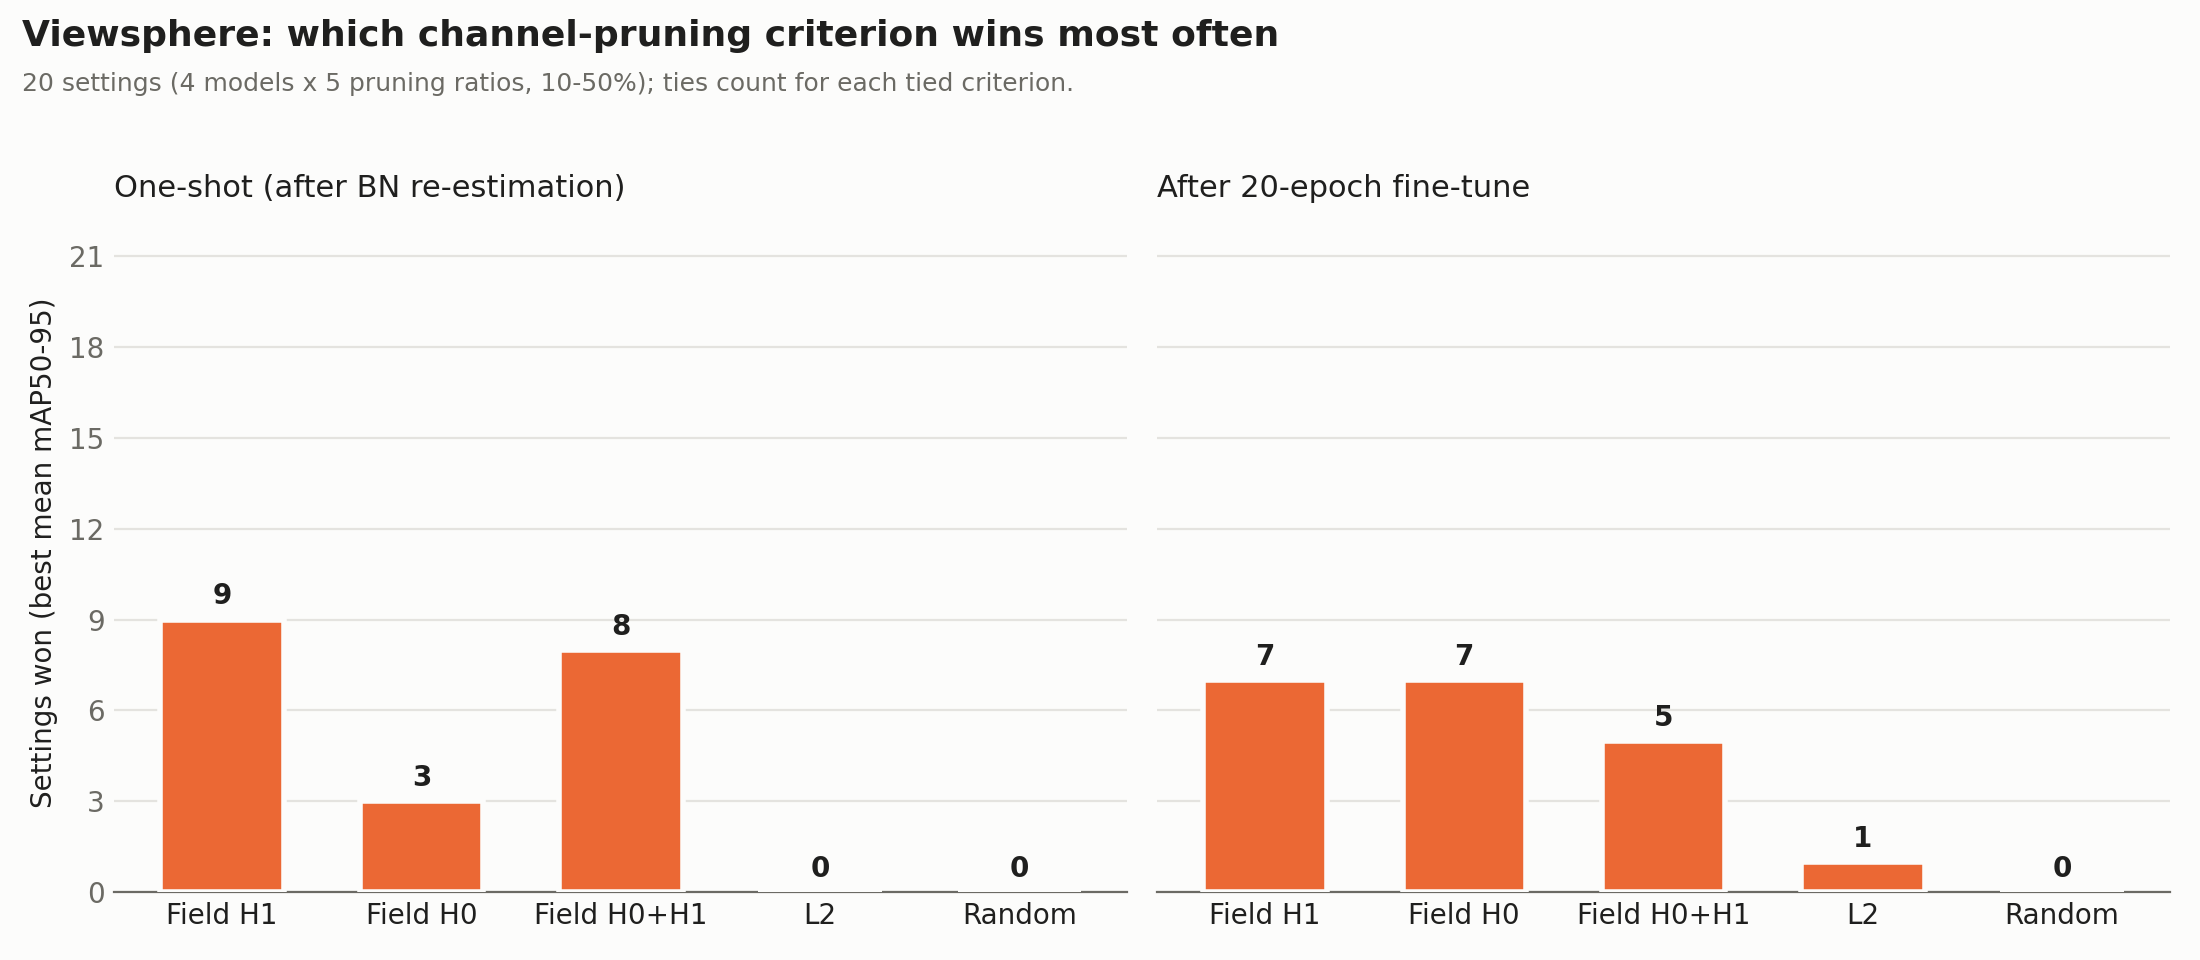
\includegraphics[width=\linewidth]{figures/criterion_wins_viewsphere.png}
\tnote{One-shot, a persistence score wins all 20 (field~H1 9, H0+H1 8, H0 3); after fine-tuning, 19
of 20 (field~H1 and H0 7 each, H0+H1 5), L2 1.}
\end{figure}

\begin{figure}[H]
\centering
\caption{Viewsphere v2: which channel-pruning criterion wins most often}
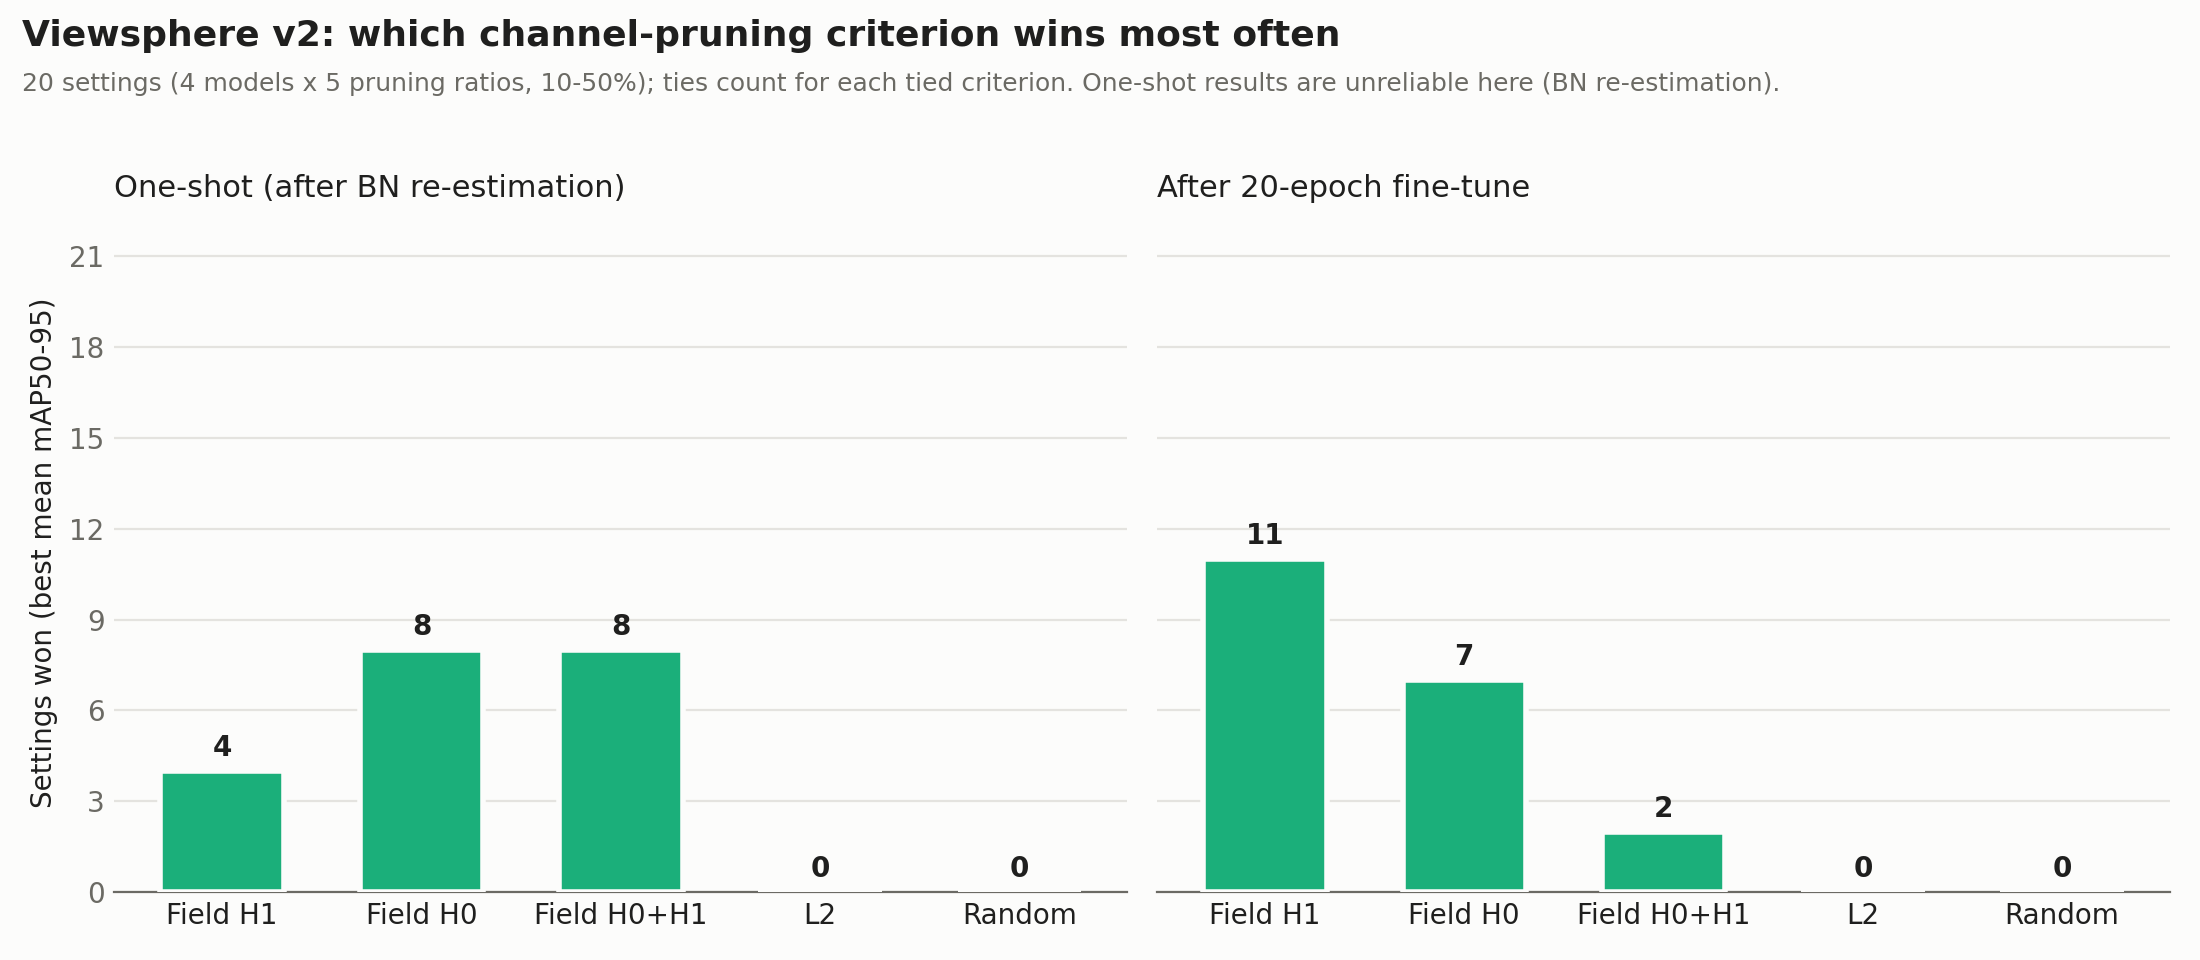
\includegraphics[width=\linewidth]{figures/criterion_wins_viewsphere2.png}
\tnote{A persistence score wins all 20 settings, one-shot (field~H0 and H0+H1 8 each, H1 4) and after
fine-tuning (field~H1 11, H0 7, H0+H1 2).}
\end{figure}

\begin{figure}[H]
\centering
\caption{COCO: which channel-pruning criterion wins most often}
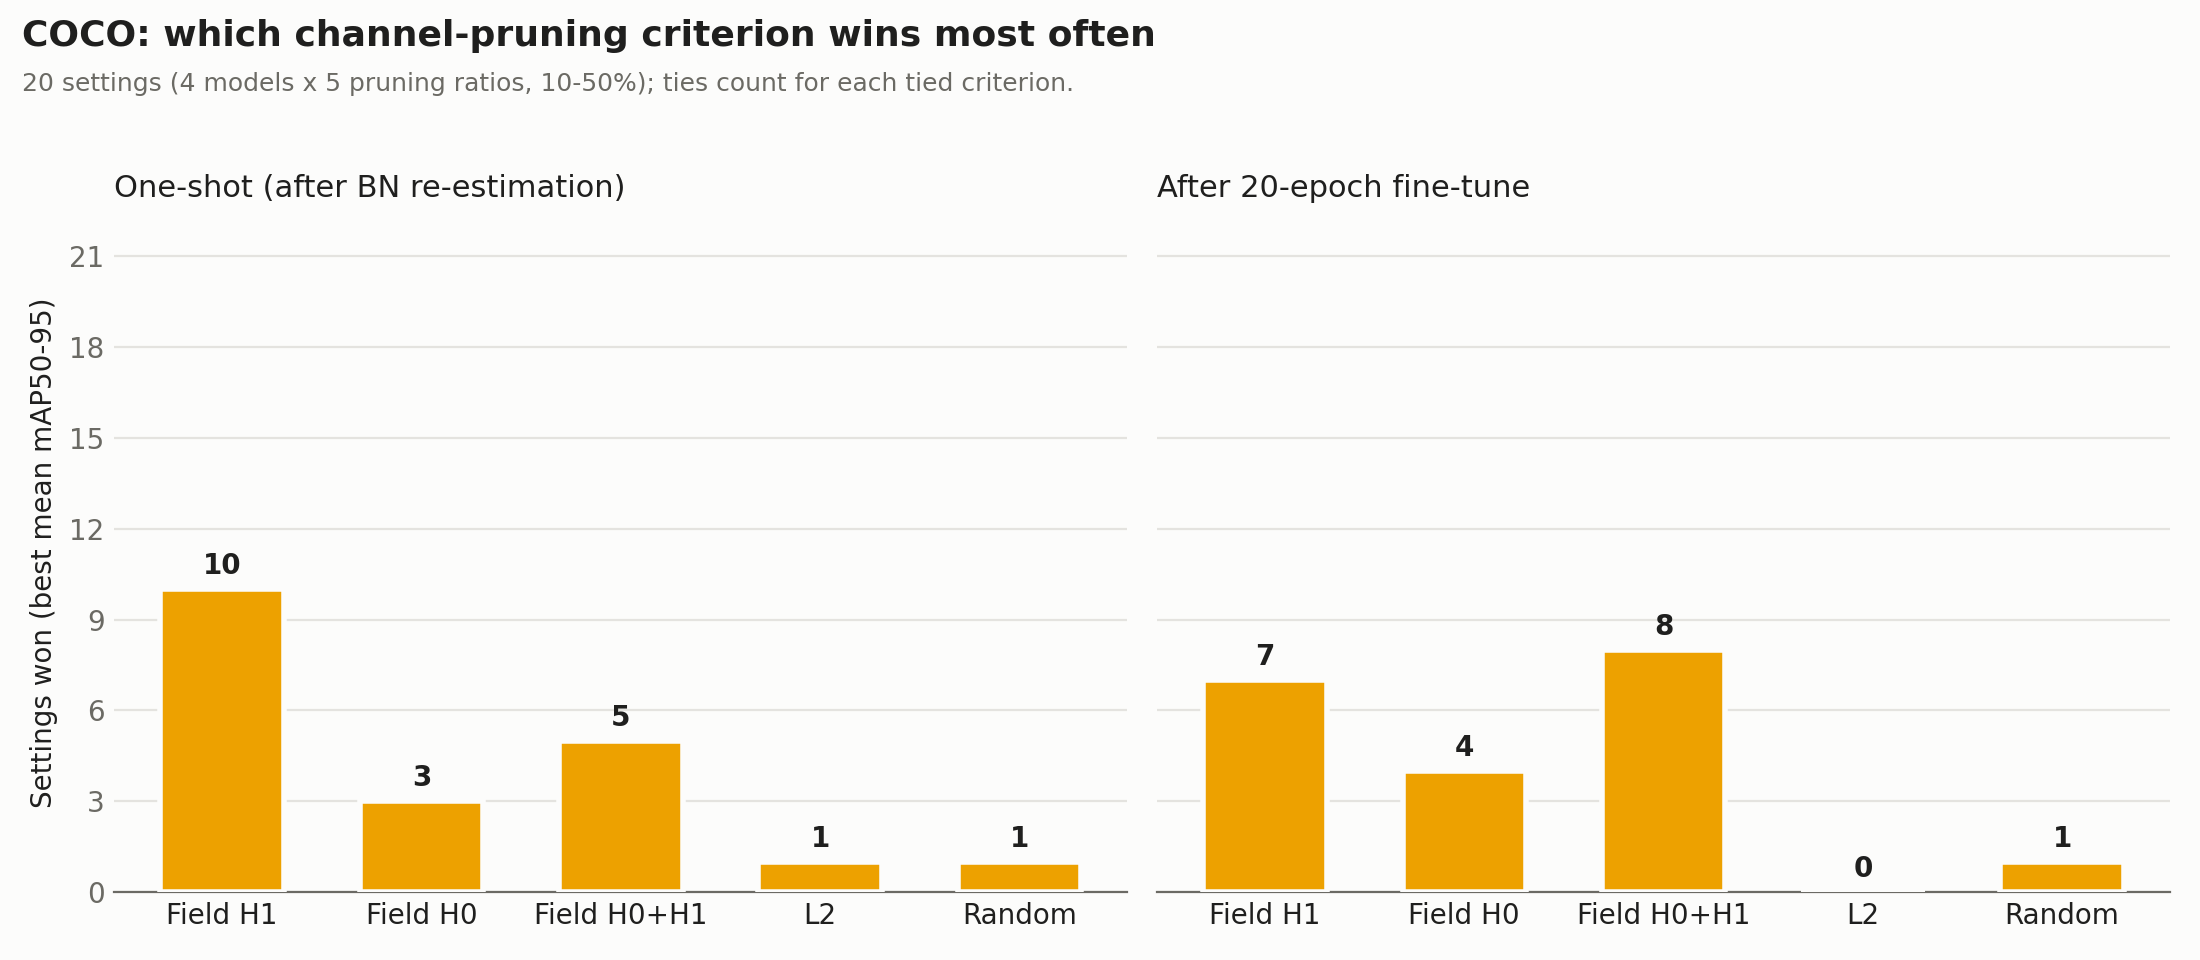
\includegraphics[width=\linewidth]{figures/criterion_wins_coco.png}
\tnote{One-shot, field~H1 wins half the settings (10 of 20). After fine-tuning a persistence score wins
19 of 20 (field~H0+H1 8, field~H1 7, field~H0 4); L2 wins none.}
\end{figure}

\begin{figure}[H]
\centering
\caption{All datasets: which channel-pruning criterion wins most often}
\label{fig:wins}
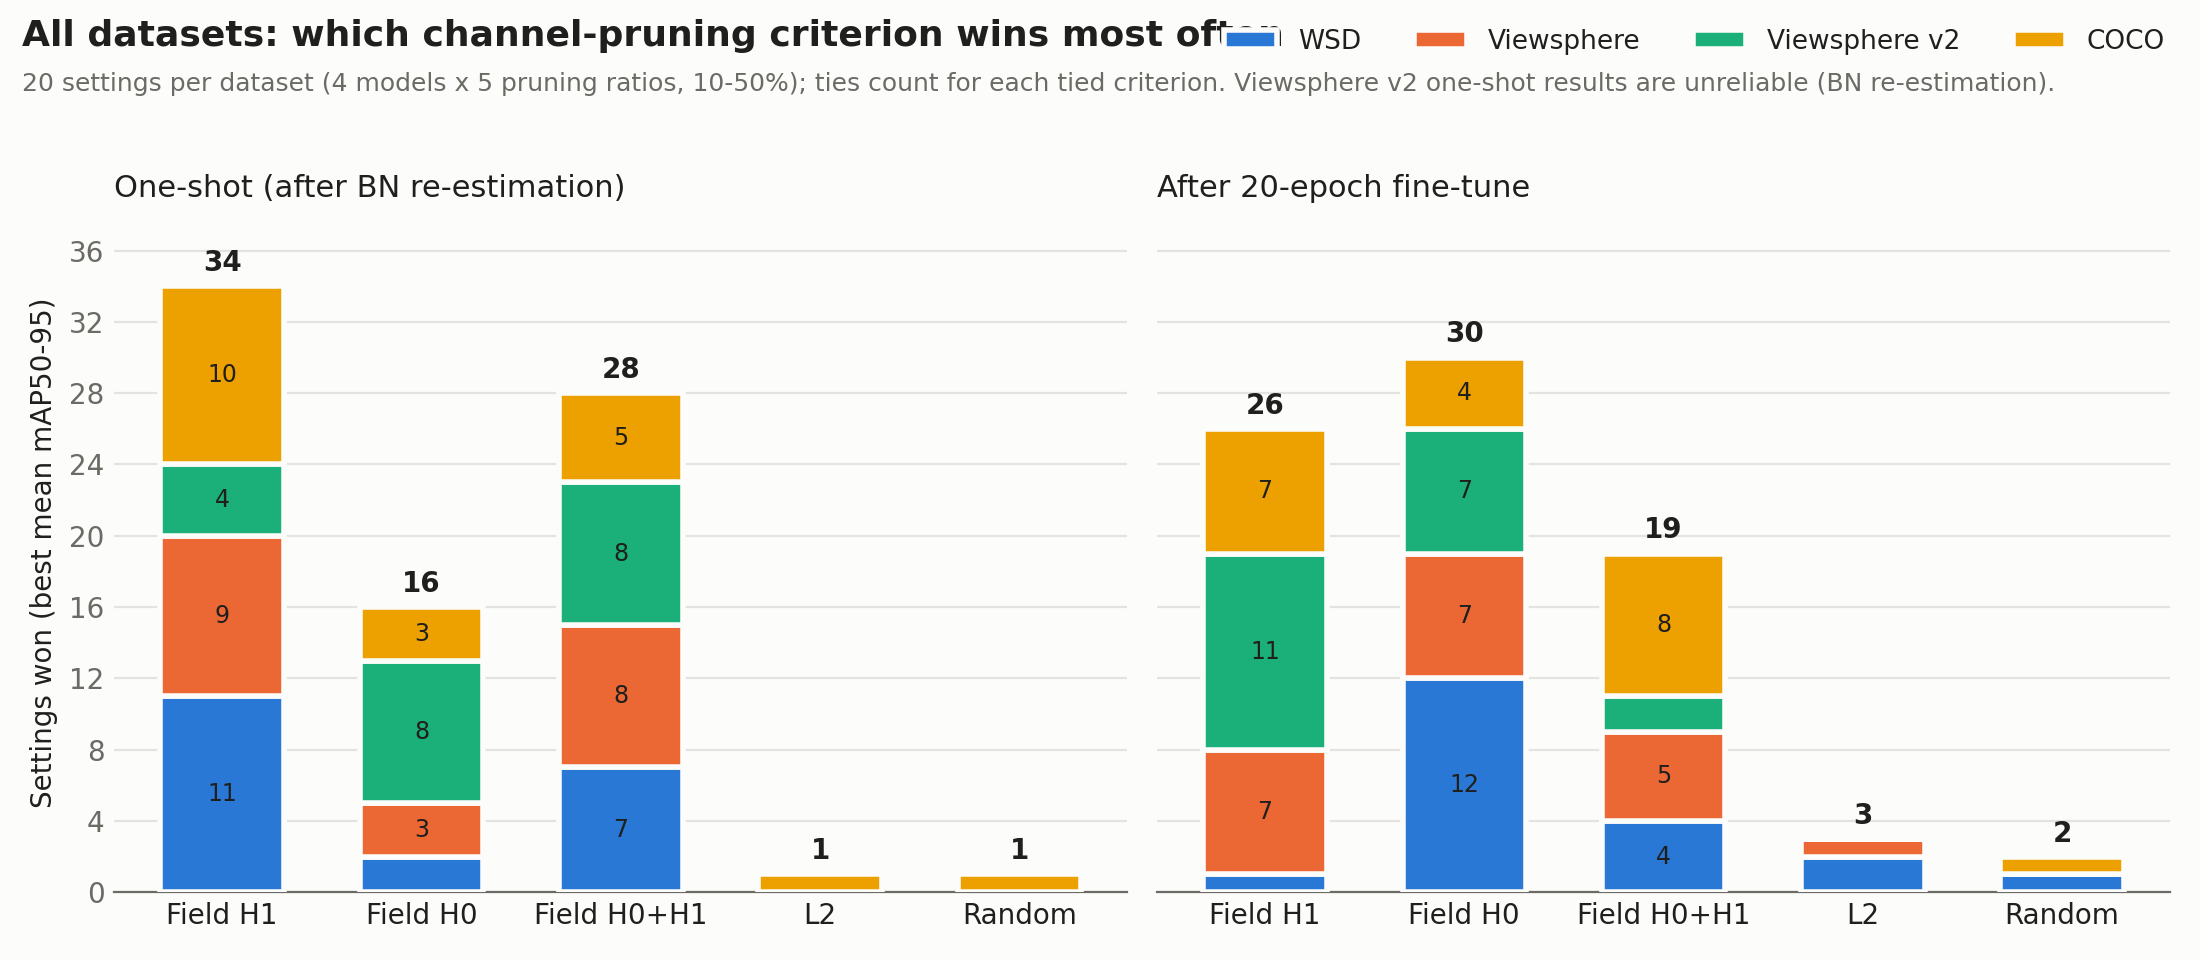
\includegraphics[width=\linewidth]{figures/criterion_wins.png}
\tnote{Figures~\ref{fig:w-wsd}--\ref{fig:wins} stacked. One-shot, a persistence score wins 78 of 80
(field~H1 34, H0+H1 28, H0 16); L2 and random win 1 each, both on COCO. After fine-tuning, 75 of 80
(field~H0 30, H1 26, H0+H1 19); L2 wins 3 and random 2.}
\end{figure}

Win counts say which criterion is best, not by how much. Figure~\ref{fig:gapl2} shows the margin: how
far each persistence score is from L2 at each pruning ratio.

\begin{figure}[H]
\centering
\caption{How close the persistence scores are to L2}
\label{fig:gapl2}
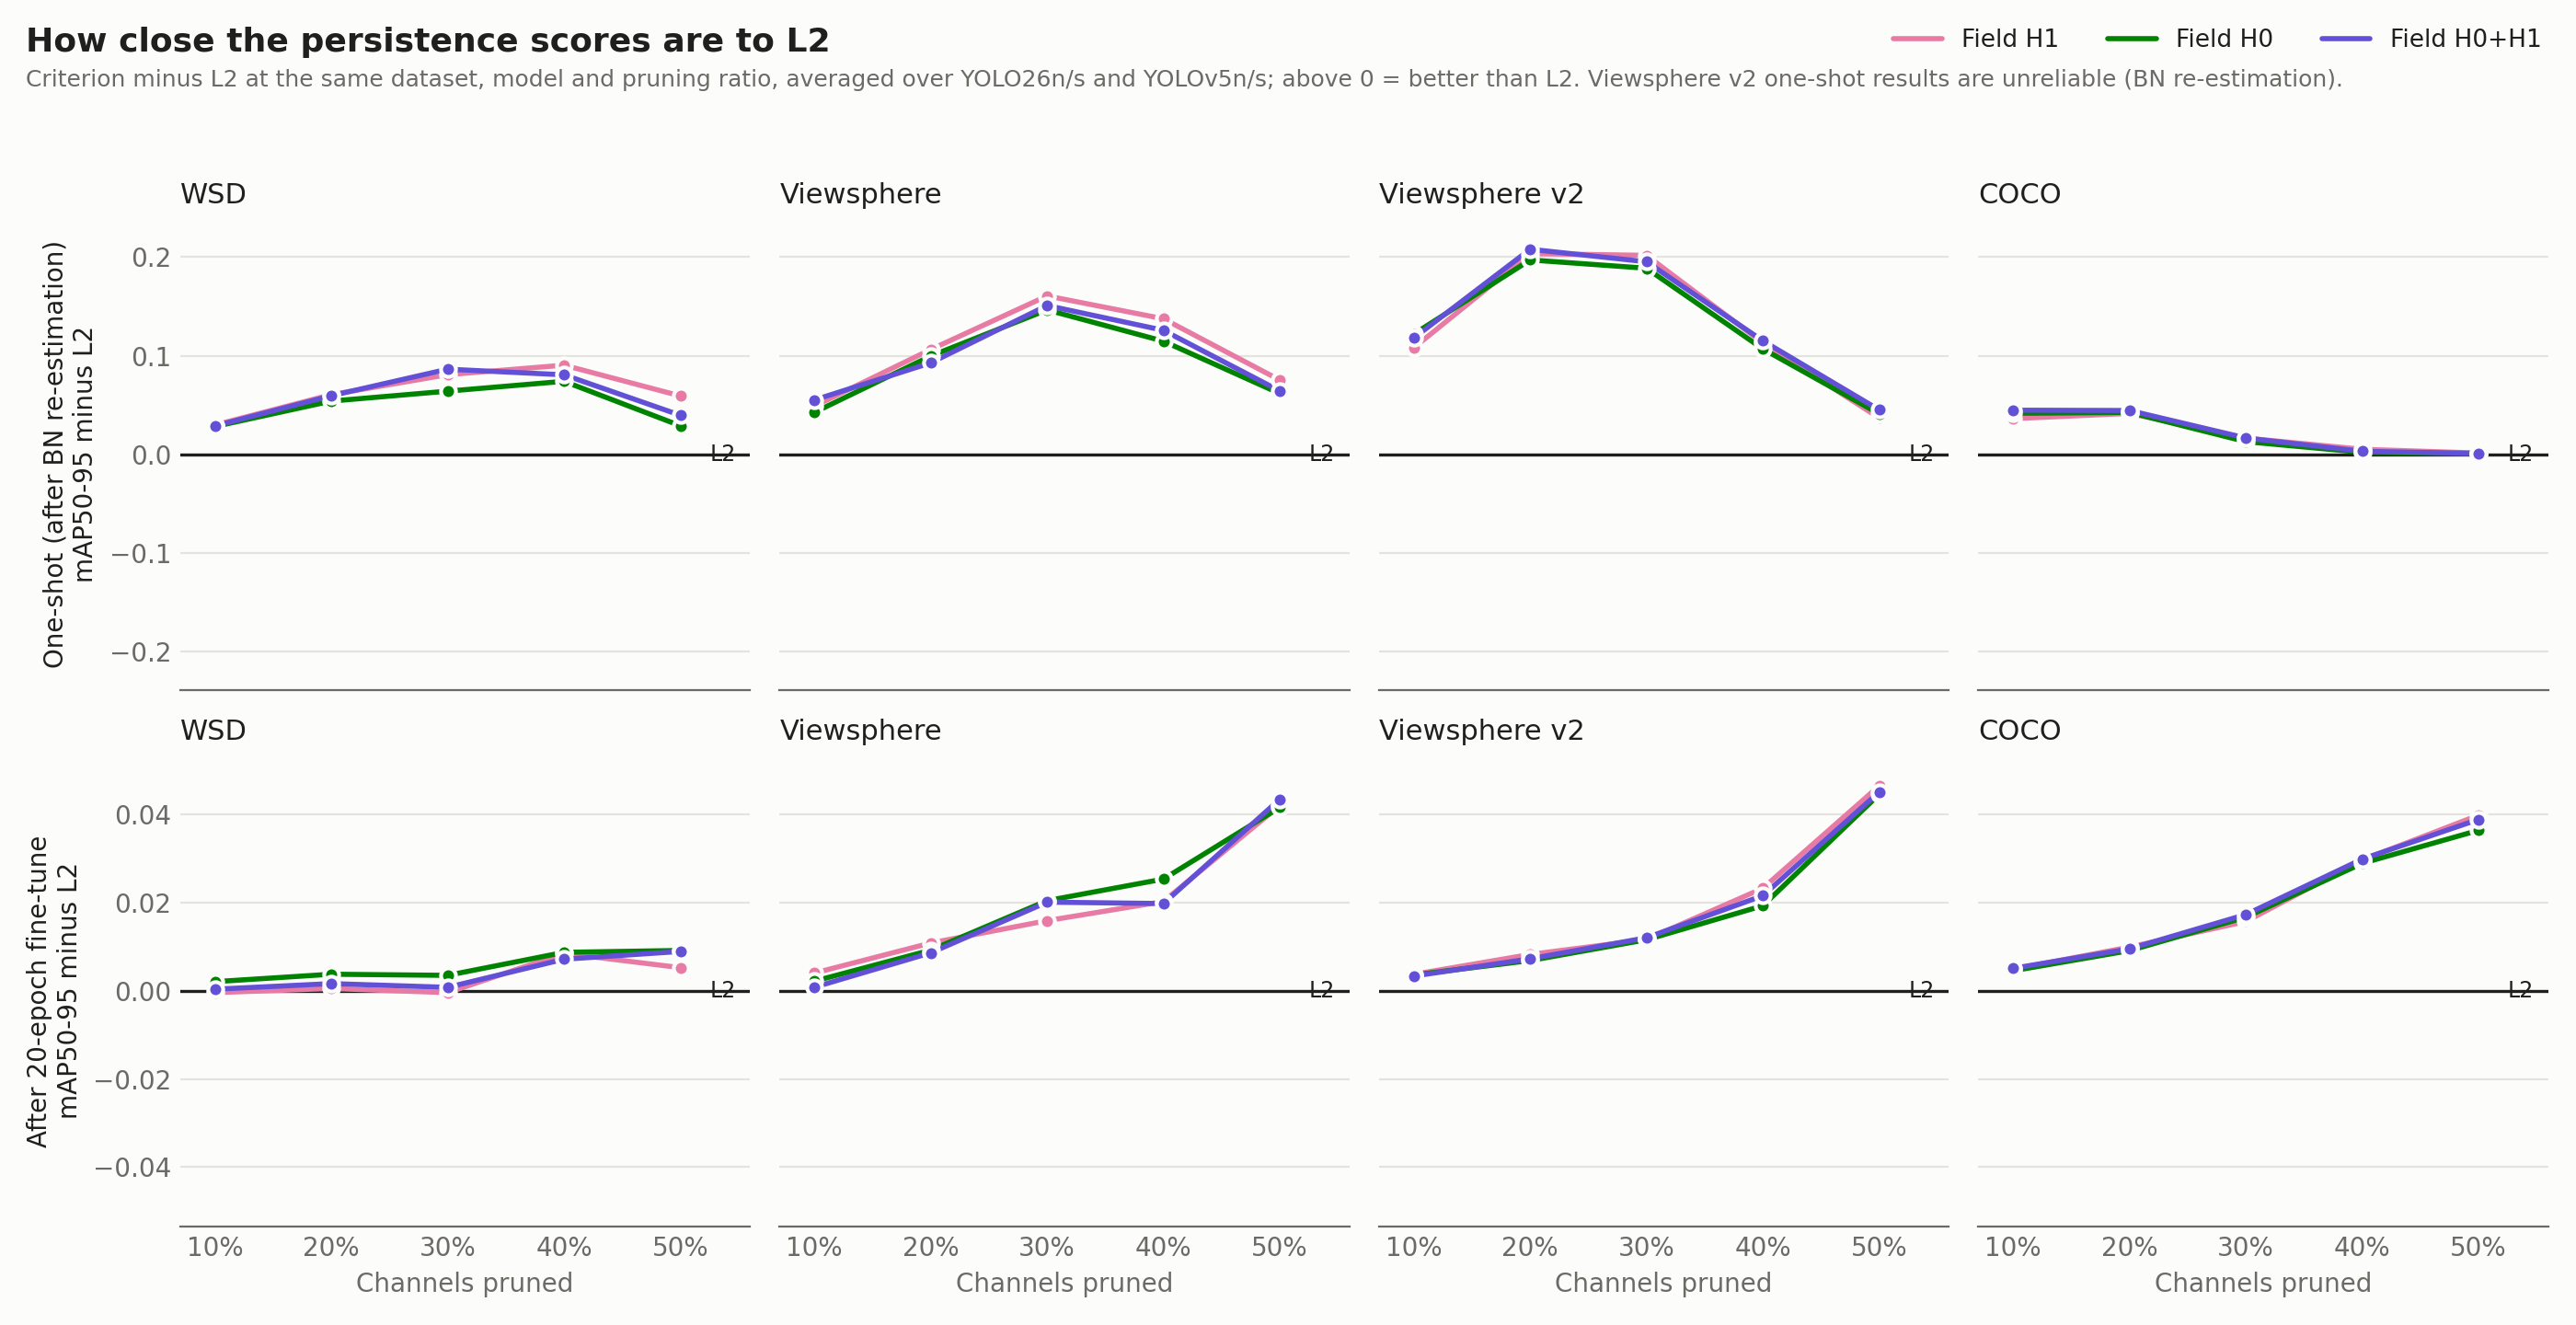
\includegraphics[width=\linewidth]{figures/gap_to_l2.png}
\tnote{Criterion mAP50-95 minus L2's at the same dataset, model and pruning ratio, averaged over
YOLO26n/s and YOLOv5n/s; 0 = L2, above = better. The three persistence scores move together, mostly
within 0.01 of each other. One-shot, they lead L2 on every dataset: by up to 0.09 on WSD (at
30--40\%), 0.16 on Viewsphere and 0.21 on Viewsphere~v2 (at 20--30\%), and on COCO by about 0.04 at
10--20\%, shrinking to 0 by 50\% (where every criterion is near zero). After fine-tuning they are level
with L2 on WSD (within 0.01) and ahead elsewhere by a margin that grows with pruning, from +0.001--0.005
at 10\% to about +0.04 at 50\% on Viewsphere, Viewsphere~v2 and COCO. The averages hide model-to-model
variation, and many of the small gaps are within seed noise.}
\end{figure}

%======================================================================
\section{Datasets}
\label{sec:data}

\begin{table}[H]
\centering\small
\caption{Datasets and the starting models that are pruned}
\adjustbox{max width=\linewidth}{%
\begin{tabular}{llll}
\toprule
Dataset & Content & Train / val images & Starting model \\
\midrule
WSD v71 & satellite components: antenna, body, solar, thruster & 1,005 / 186 & COCO YOLO26n/s fine-tuned on it \\
Viewsphere & 4 rendered satellites, relabelled to WSD's 4 classes & 925 / 160 & COCO YOLO26n/s fine-tuned on it, pixel noise \\
Viewsphere v2 & 17 rendered satellites, same classes and split (Section~\ref{sec:vs2}) & 4,079 / 680 & COCO YOLO26n/s fine-tuned on it, pixel noise \\
COCO 2017 & 80 everyday object classes & 10k subset / 5,000 & Ultralytics pretrained YOLO26n/s \\
\bottomrule
\end{tabular}}
\end{table}

\textbf{Viewsphere} renders Clementine, ICESatB, Jason-1 and Sentinel-6 from 18 viewing angles,
4 distances and 5 Sun phases; it is split by viewing angle, and frames with less than 10\% of the
satellite lit are dropped from train. On \textbf{COCO}, pruned models are fine-tuned on a fixed
10k-image subset of train2017, so the unpruned model given the same fine-tune is the reference.

\textbf{Starting models.} On every dataset the model that is pruned is Ultralytics' COCO-pretrained
YOLO26n/s (or YOLOv5n/s, Section~\ref{sec:v5}) fine-tuned on that dataset; best validation mAP50-95
0.419 / 0.451 on WSD, 0.613 / 0.630 on Viewsphere and 0.492 / 0.520 on Viewsphere~v2 (YOLO26n/s).
These replace the earlier WSD models trained from scratch (0.37--0.41) and the Viewsphere models
fine-tuned from them; the COCO start was also better on the test split in 7 of 8 cases. The renders
are about 96\% exactly-black pixels (WSD: 38\%), and models trained on them become hypersensitive to
tiny noise on the background (Section~\ref{sec:vs2}). Every Viewsphere fine-tune (the starting models
and all pruning fine-tunes) therefore adds Gaussian pixel noise, with a standard deviation drawn per
image between 0 and 3 gray levels, and so do the images used to re-estimate BatchNorm statistics.
WSD needs none.

%======================================================================
\section{Methods}

\textbf{Channel pruning.} In every convolution from layer 6 on (the stem, the detection head and
attention layers are left alone), the lowest-scoring 10--50\% of channels are removed physically.
All criteria remove the same number of channels per layer, so they give equally sized models; at
50\% that is $-$39\% parameters and $-$28\% GFLOPs. The criteria compared:
\begin{itemize}
\item \textbf{PEEK field~H1} --- builds the layer's PEEK map (pseudo-entropy of the activations
  across channels at each pixel), measures its loops (H1 persistent homology), and removes first the
  channels whose absence changes that topology least. Scored on 128 training images.
\item \textbf{PEEK field~H0} and \textbf{field~H0+H1} --- the same, but measuring the map's
  connected components (H0) or the total persistence of both (H0+H1).
\item \textbf{L2} --- removes the filters with the smallest weight magnitude.
\item \textbf{Random} --- removes a random set of channels; the baseline to beat.
\end{itemize}

\textbf{Block replacement.} Whole C3k2 blocks are swapped for a 1$\times$1 convolution, $k = 1, 2, 3$
blocks at a time, ranked by the persistence of each block's PEEK map: \emph{head} ranks the four
head blocks on raw scores; \emph{grid} and \emph{null} rank all eight C3k2 blocks with the scores
normalised for map size. Each ranking is scored three ways: \emph{C}, the 50/50 blend of
normalised H0 (secondary-peak prominence) and H1 (pocket persistence) used so far, \emph{H0} only,
or \emph{H1} only. As a non-topological baseline, \emph{L2} ranks blocks by the RMS of their
convolution weights (lowest cut first), over the head blocks or over all eight blocks without
normalisation (\emph{all, raw}); it is not run on COCO. A cut set picked by several rankings is trained
once. The baseline to beat is 23 random block orders.

\textbf{Measurements} (mAP50-95 on the validation split):
\begin{itemize}
\item \textbf{One-shot} --- right after pruning, with only the BatchNorm statistics re-estimated;
  10 seeds (random: 10 different masks).
\item \textbf{After a 20-epoch fine-tune} --- AdamW, batch 16; lr $1.25\times10^{-3}$ (WSD,
  Viewsphere) or $1.25\times10^{-4}$ (COCO); 5 seeds. Block cuts get the same fine-tune, 3 seeds.
\item \textbf{Recovery} --- separate fine-tunes stopped after 250 to 5,000 batches; 3 seeds on WSD
  and Viewsphere, 1 on COCO (which also has runs on all of train2017).
\end{itemize}
A difference is treated as real when it exceeds two standard errors across seeds (roughly a 95\%
test); otherwise it is within seed noise.

%======================================================================
\section{Results}

Each dataset has a channel-pruning table; recovery (Tables~\ref{tab:rec}--\ref{tab:speed}) and
block replacement (Tables~\ref{tab:blockgap} and~\ref{tab:blocks}) are collected for all three at
the end of this section.

\subsection{WSD}

\begin{table}[H]
\centering\small
\caption{WSD: channel pruning by criterion}
\label{tab:wsd}
\tbl{wsd_channel}
\tnote{mAP50-95 on the validation split, mean over seeds (one-shot: 10, fine-tuned: 5).
\textbf{Bold} = best criterion; $^\dagger$ = its lead over the runner-up holds up across
seeds.}
\end{table}

\begin{itemize}
\item \textbf{One-shot:} a persistence score is best at every ratio, ahead of L2 by 0.04--0.13
  wherever anything survives (field~H1 0.319 vs 0.275 at 10\% on n; 0.135 vs 0.019 at 50\% on s), and
  L2 is barely above random. (With the earlier from-scratch models, L2 led here.) At 50\% on n every
  criterion is below 0.02.
\item \textbf{After fine-tuning:} all criteria end within 0.01 of each other at every ratio (50\%:
  0.355--0.363 on n, 0.399--0.409 on s). Field~H0 has the highest mean at 30--50\% on both models, but
  no lead holds up. At 50\% the pruned models are 0.04--0.05 below the unpruned ones.
\item \textbf{H0 and H0+H1:} one-shot, H0+H1 edges out field~H1 at 30\% on n and at 10\% on s, while
  field~H1 is best at 50\%; after fine-tuning the three are within 0.008 of each other.
\item \textbf{Recovery:} at 50\%, the persistence scores lead L2 and random by 0.02--0.06 after 250
  batches (4 epochs); by 1,000 batches random has caught up, and at 5,000 all criteria are within 0.01
  of each other and 0.03--0.04 below unpruned. 10\% pruning reaches 95\% of the unpruned model within
  250--500 batches; 50\% never does within 5,000.
\item \textbf{Blocks:} scored on H1 alone, the null ranking beats random choice at every $k$ on both
  models (+0.006 to +0.033) and gives the best cut at every $k$ (on n at $k = 2$, 0.400 vs 0.405 uncut).
  The blended grid ranking, the best one with the earlier models, is now worse than random at
  $k = 2, 3$ ($-$0.012 to $-$0.036). L2 over all blocks beats random at $k = 2$ (+0.014, +0.015) but
  not at $k = 3$.
\end{itemize}

\subsection{Viewsphere}

\begin{table}[H]
\centering\small
\caption{Viewsphere: channel pruning by criterion}
\tbl{viewsphere_channel}
\tnote{mAP50-95 on the validation split, mean over seeds. Bold and $^\dagger$ as in
Table~\ref{tab:wsd}.}
\end{table}

\begin{itemize}
\item \textbf{One-shot:} the persistence scores lead by a wide margin, and L2 is no better than
  random: at 30\%, 0.17--0.20 vs 0.04 (L2) and 0.02 (random) on n, 0.32--0.37 vs 0.18 and 0.19 on s.
\item \textbf{After fine-tuning:} all within 0.01 at 10\%, but the persistence scores pull ahead
  with pruning: at 50\%, 0.510--0.522 vs 0.431 (L2) and 0.450 (random) on n, 0.584--0.585 vs 0.554 and
  0.564 on s.
\item \textbf{H0 and H0+H1:} one-shot, H0+H1 is the best of the three on n and field~H1 from 30\% on s;
  after fine-tuning the three are within 0.012, and H0+H1's lead at 50\% on n (0.522) is the only one
  that holds up.
\item \textbf{Recovery:} at 50\% the persistence scores lead L2 and random at every budget, most of all
  early (1,000 batches, n: 0.50--0.52 vs 0.41--0.42), and still at 5,000 (0.557--0.568 vs 0.538--0.539
  on n; 0.615--0.617 vs 0.602--0.608 on s). YOLO26s at 50\% is back to 95\% of the unpruned model after
  2,500 batches with every persistence score (L2: never; random: 5,000); YOLO26n stays 0.05 behind.
\item \textbf{Blocks:} the raw head ranking beats random choice at every $k$ on both models (+0.015 to
  +0.020), and so does L2 over all blocks (+0.020 to +0.038), which gives the best cuts at $k = 2, 3$.
  The size-normalised grid and null rankings are mostly worse than random (down to $-$0.063); scored
  on H1 alone, null is level with random or better (up to +0.027).
\end{itemize}

\subsection{COCO}

\begin{table}[H]
\centering\small
\caption{COCO: channel pruning by criterion}
\tbl{coco_channel}
\tnote{mAP50-95 on val2017, mean over seeds. Bold and $^\dagger$ as in Table~\ref{tab:wsd}.}
\end{table}

\begin{itemize}
\item \textbf{One-shot:} far more fragile than WSD (near zero from 30--40\%), but the order is clean:
  field~H1 $>$ L2 $>$ random at every ratio, and every lead holds up.
\item \textbf{After fine-tuning:} the same order survives and the gap grows with pruning; at 50\%,
  field~H1 0.187 vs L2 0.126 vs random 0.104 (n) and 0.276 vs 0.212 vs 0.203 (s).
\item \textbf{H0 and H0+H1:} also ahead of L2 at every ratio after fine-tuning, and within 0.012
  of field~H1. One-shot, field~H1 is the best of the three from 30\% on (field~H0 at 10\% on n);
  after fine-tuning, field~H1's lead at 50\% on n (0.187 vs 0.175 and 0.178) holds up.
\item \textbf{Recovery:} the 10k subset caps it, and field~H1 recovers fastest. On all of train2017
  (7 epochs), 10\% pruning reaches 96--97\% of the unpruned model and 50\% reaches 73--83\%, with
  field~H1 still about 0.02 ahead of L2.
\item \textbf{Blocks:} the null ranking is best on YOLO26n (at $k = 3$, 0.265 vs a random median of
  0.144), grid on YOLO26s at $k \le 2$; scored on H0 alone, null beats random at every $k$ on
  YOLO26s (+0.033 to +0.063), while H1 alone is worse than random at $k = 1$. One cut block already
  costs 0.025--0.06 mAP.
\end{itemize}

\subsection{Recovery, all datasets}

\textbf{Which criterion recovers first?} After 50\% pruning the persistence scores lead L2 and random
early on every dataset. On WSD the lead is gone by 1,000 batches, and at 5,000 all criteria are
within 0.01. On Viewsphere it shrinks but lasts to 5,000 batches (0.01--0.03). On COCO, field~H1
leads at every budget at 30--50\% pruning, most of all early (50\%, 1,000 batches, YOLO26n: 0.077 vs
0.039 vs 0.022), and still after 7 epochs on all of train2017 (Table~\ref{tab:reclong}). Light
pruning (10\%) reaches 95\% of the unpruned model within 250--500 batches on WSD and Viewsphere, but on
COCO only after 3--7 epochs on the full training set; 50\% gets there within 5,000 batches only on
Viewsphere YOLO26s, and 30--50\% never on COCO (Table~\ref{tab:speed}). The three persistence scores
recover alike: on COCO all three stay well ahead of L2 at 50\% (1,000 batches, YOLO26n: 0.072 and
0.076 vs 0.077 for field~H1), and on WSD and Viewsphere they are mostly within 0.01 of each other.

\begin{table}[H]
\centering\small
\caption{Recovery after channel pruning, by training budget}
\label{tab:rec}
\tbl{recovery}
\tnote{mAP50-95 after separate fine-tunes of 250 to 5,000 batches (WSD, Viewsphere: mean of 3
seeds; COCO: 1 seed on the 10k subset). One epoch is 63 / 58 / 625 batches. \textbf{Bold} = best
criterion at that ratio and budget.}
\end{table}

\begin{table}[H]
\centering\small
\caption{COCO: recovery with longer fine-tunes}
\label{tab:reclong}
\tbl{recovery_coco_long}
\tnote{mAP50-95 on val2017 (1 seed). 25,000 and 50,000 batches on the 10k subset; \emph{full 3 / 7
ep} = fine-tuned on all of train2017 (7,393 batches per epoch, so 22k / 52k batches). Bold as in
Table~\ref{tab:rec}.}
\end{table}

\begin{table}[H]
\centering\small
\caption{Training needed to reach 95\% of the unpruned model}
\label{tab:speed}
\tbl{recovery_speed}
\tnote{Smallest training budget tested after which the pruned model reaches 95\% of the unpruned
model's mAP50-95 at the same budget (WSD, Viewsphere: 3-seed means). \emph{never} = not within
5,000 batches (COCO: not within 7 epochs on all of train2017). \textbf{Bold} = fastest criterion.
The budgets are coarse steps (250, 500, 1,000, 2,500, 5,000), so ties are common and a step can
move with seed noise.}
\end{table}

Figures~\ref{fig:bw-wsd}--\ref{fig:budgetwins} count, at each training budget, which criterion
recovers best: one figure per dataset, then all four together. Both architectures are included
(YOLOv5: Section~\ref{sec:v5}; Viewsphere~v2: Section~\ref{sec:vs2}). A setting = model (YOLO26n/s,
YOLOv5n/s) $\times$ pruning ratio (10, 30, 50\%), 12 per dataset and budget; the criterion with the highest
mean mAP50-95 wins it (ties count for each), which is not necessarily a lead beyond the seed noise.
COCO's longer budgets are left out.

\begin{figure}[H]
\centering
\caption{WSD: which criterion wins at each training budget}
\label{fig:bw-wsd}
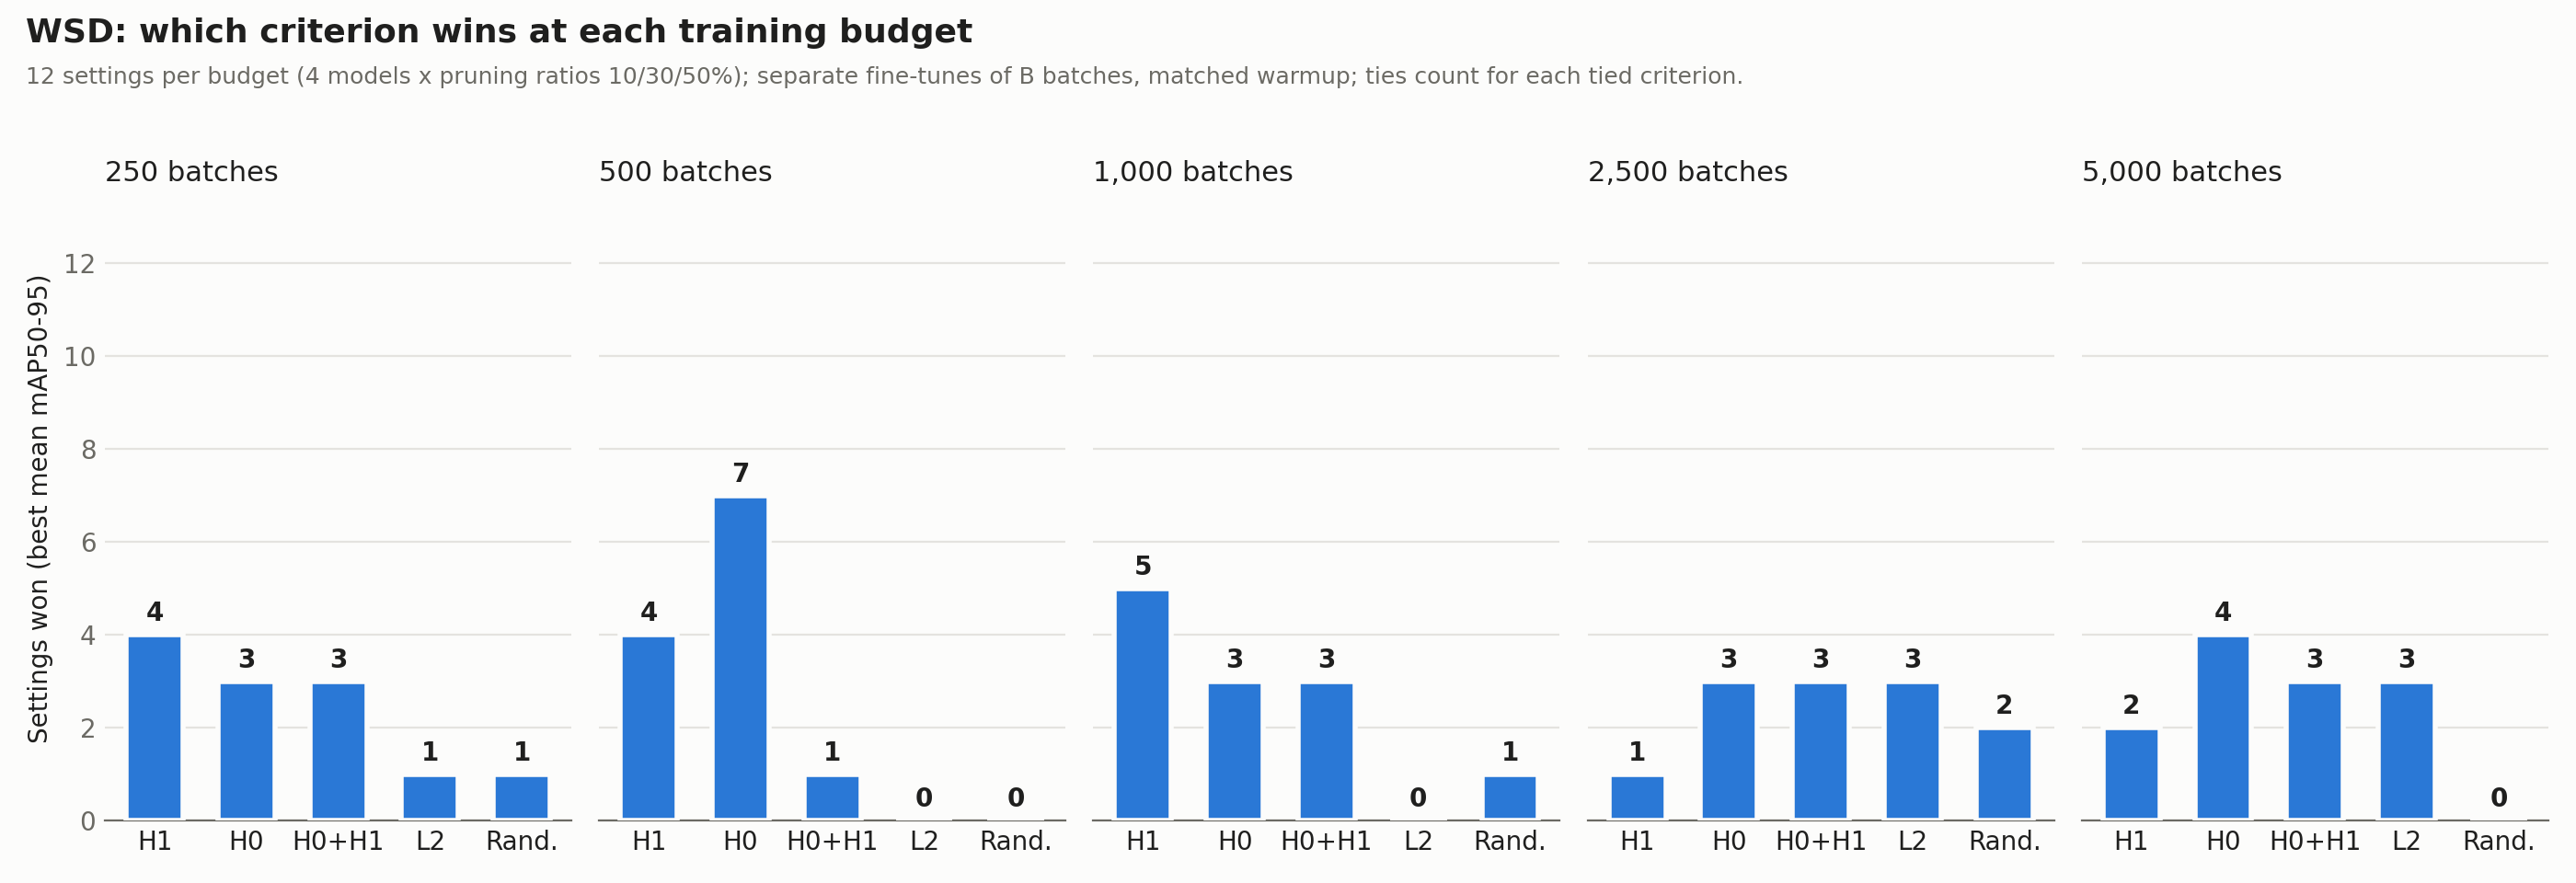
\includegraphics[width=\linewidth]{figures/budget_wins_wsd.png}
\tnote{A persistence score wins 10--12 of 12 settings up to 1,000 batches. At 2,500--5,000, when
the criteria have converged, L2 wins 3 and random up to 2.}
\end{figure}

\begin{figure}[H]
\centering
\caption{Viewsphere: which criterion wins at each training budget}
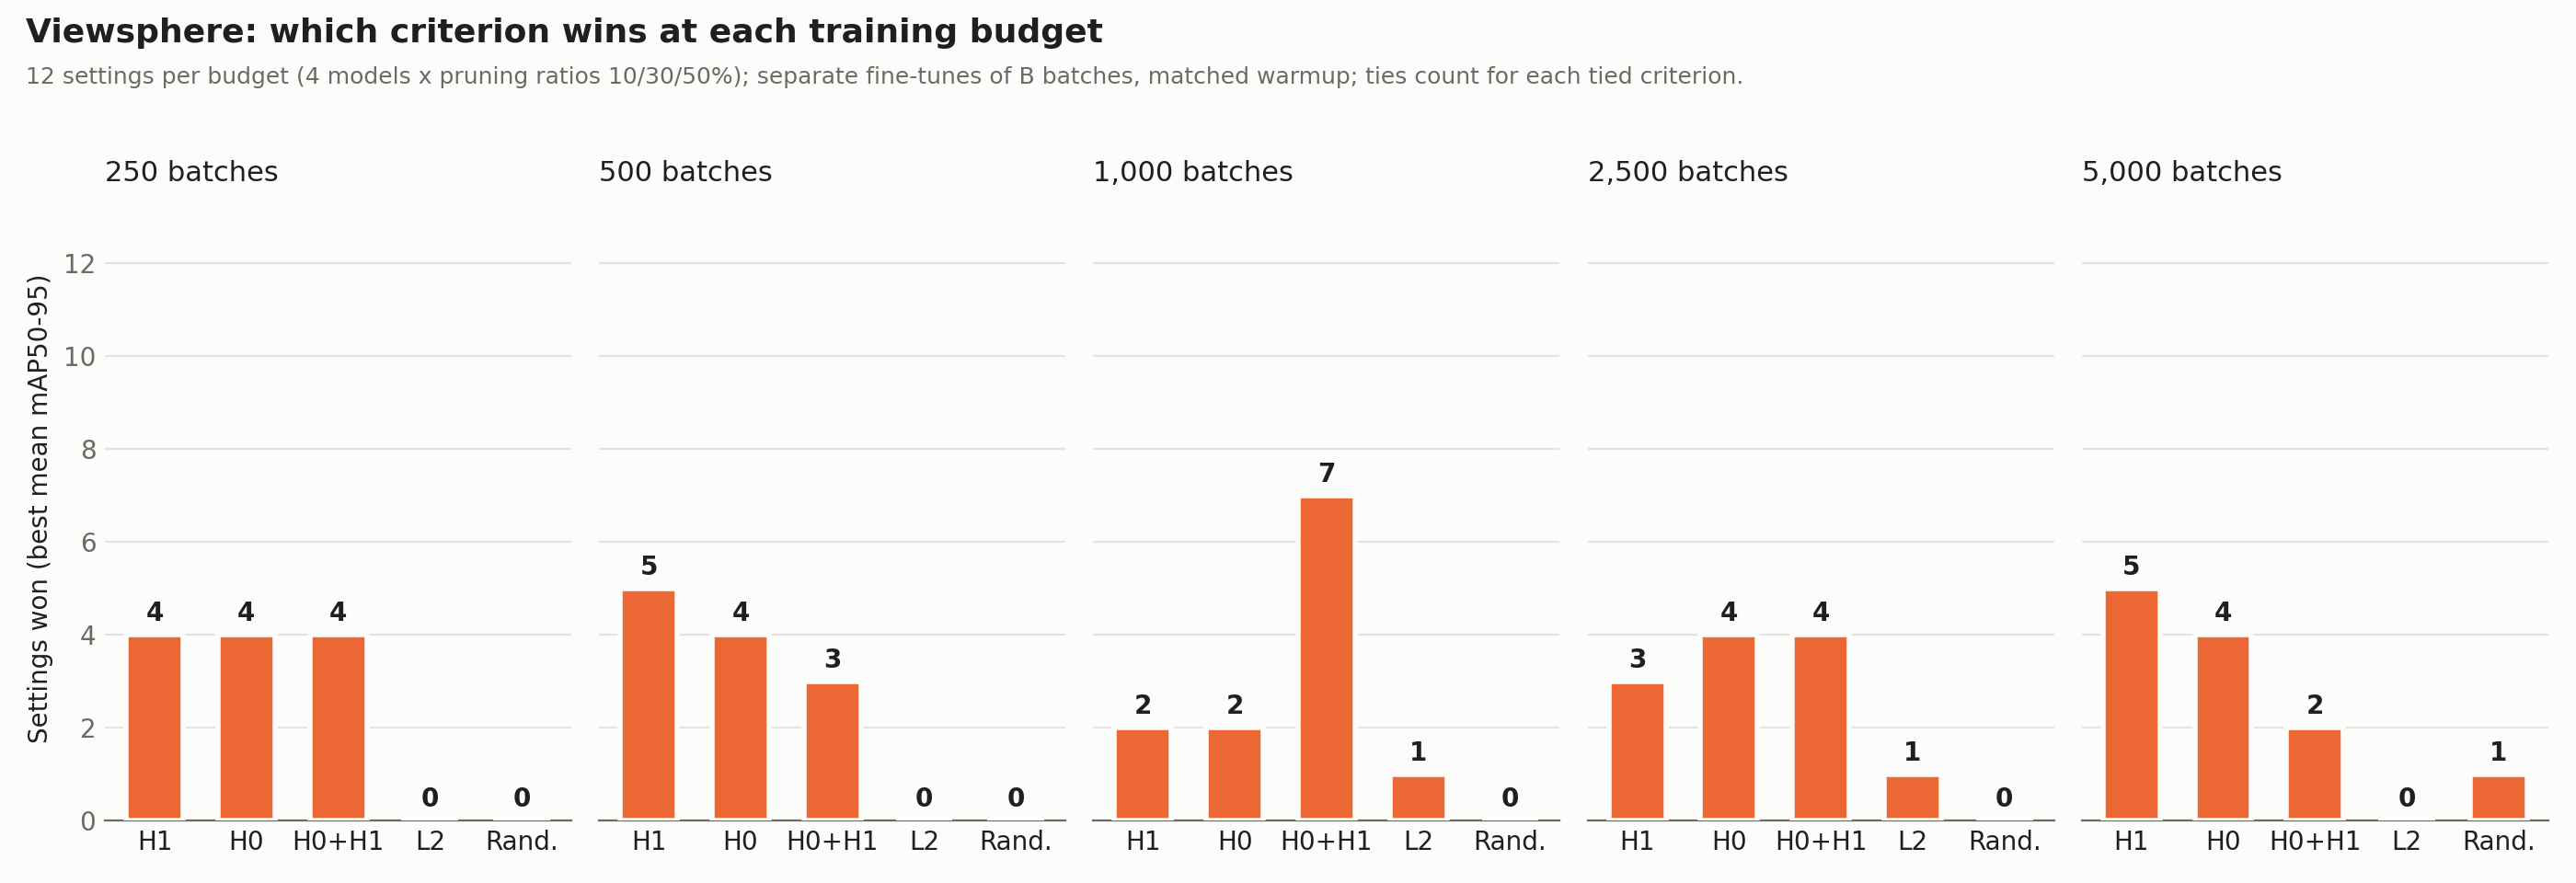
\includegraphics[width=\linewidth]{figures/budget_wins_viewsphere.png}
\tnote{A persistence score wins 11--12 of 12 settings at every budget; L2 wins 2 settings in all,
random 1.}
\end{figure}

\begin{figure}[H]
\centering
\caption{Viewsphere v2: which criterion wins at each training budget}
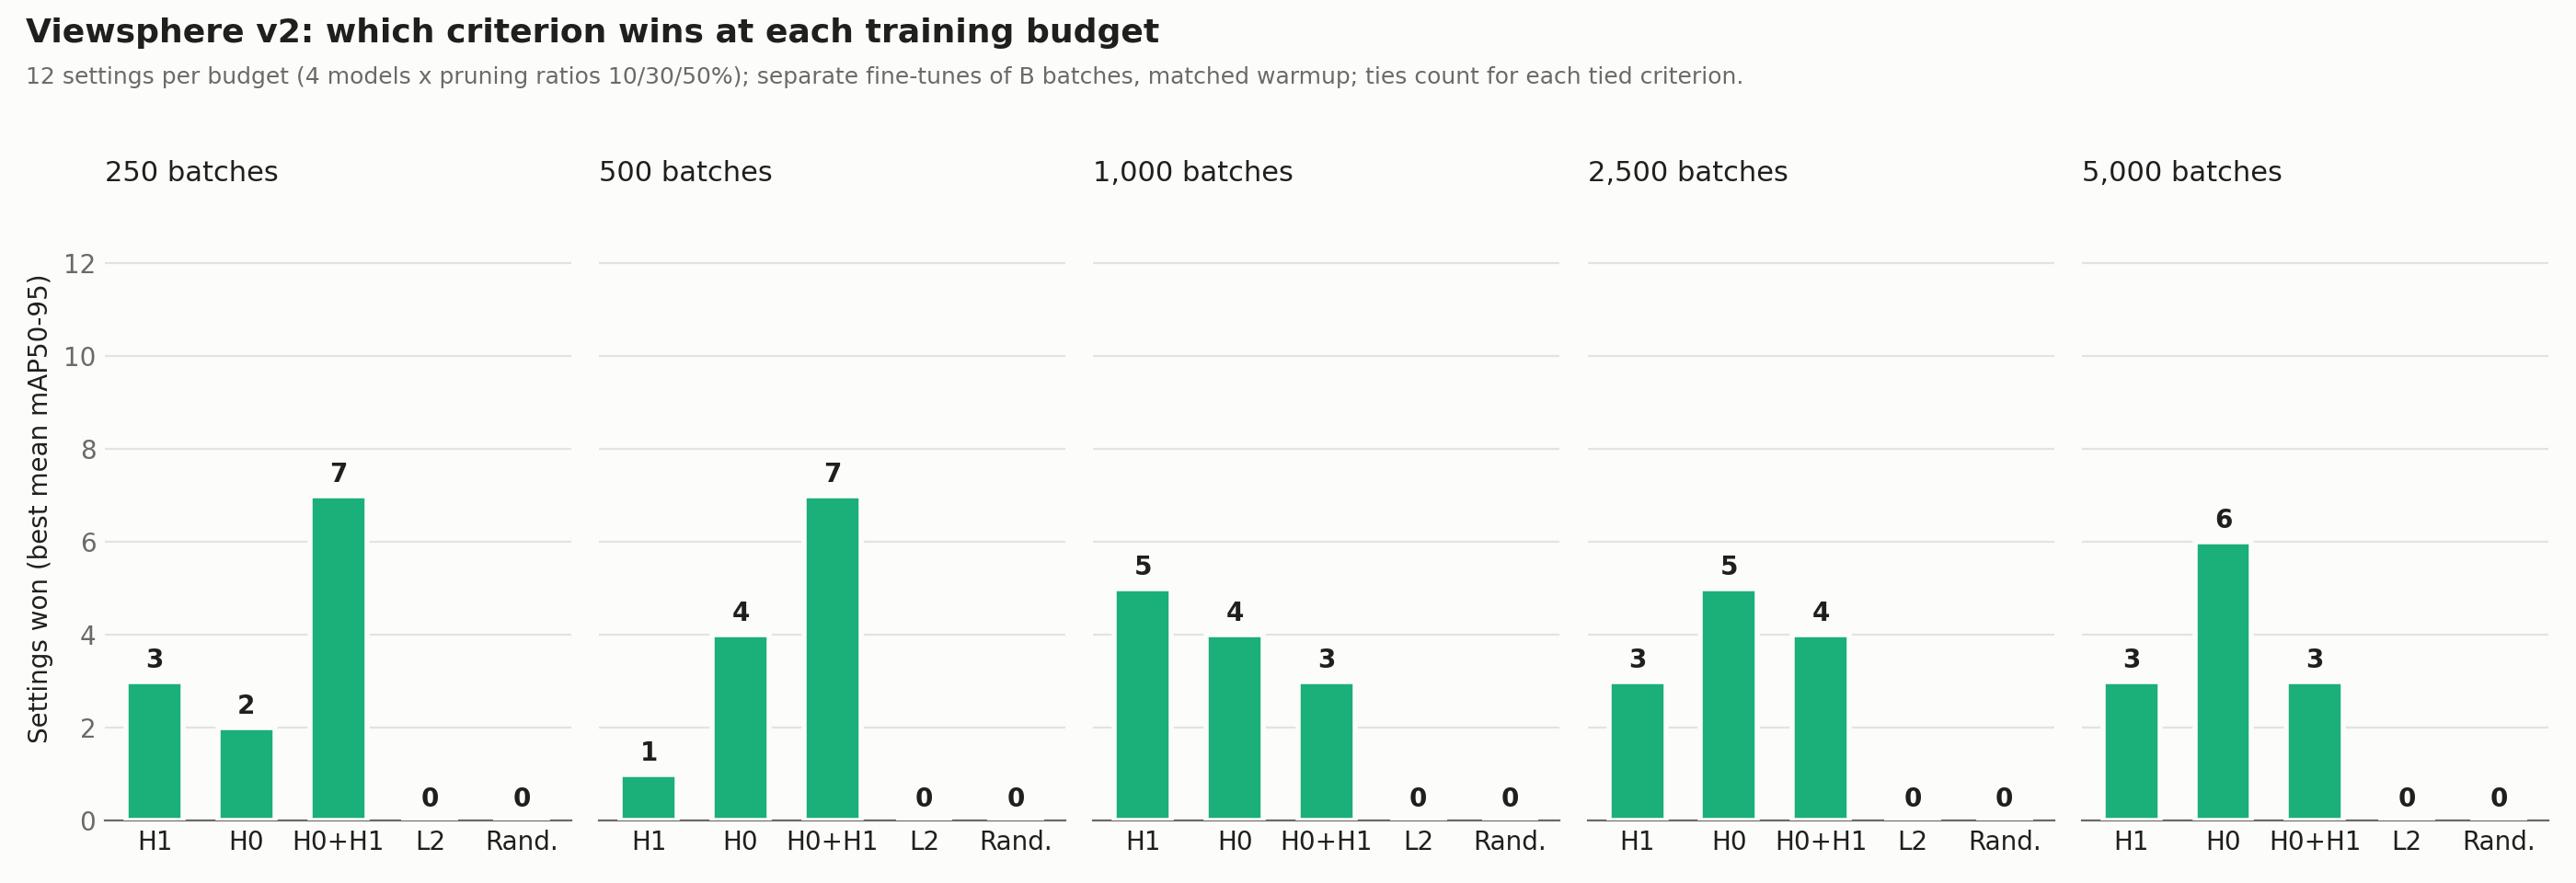
\includegraphics[width=\linewidth]{figures/budget_wins_viewsphere2.png}
\tnote{A persistence score wins every setting at every budget: field~H0+H1 most often at 250--500
batches, field~H1 at 1,000, field~H0 at 2,500--5,000.}
\end{figure}

\begin{figure}[H]
\centering
\caption{COCO: which criterion wins at each training budget}
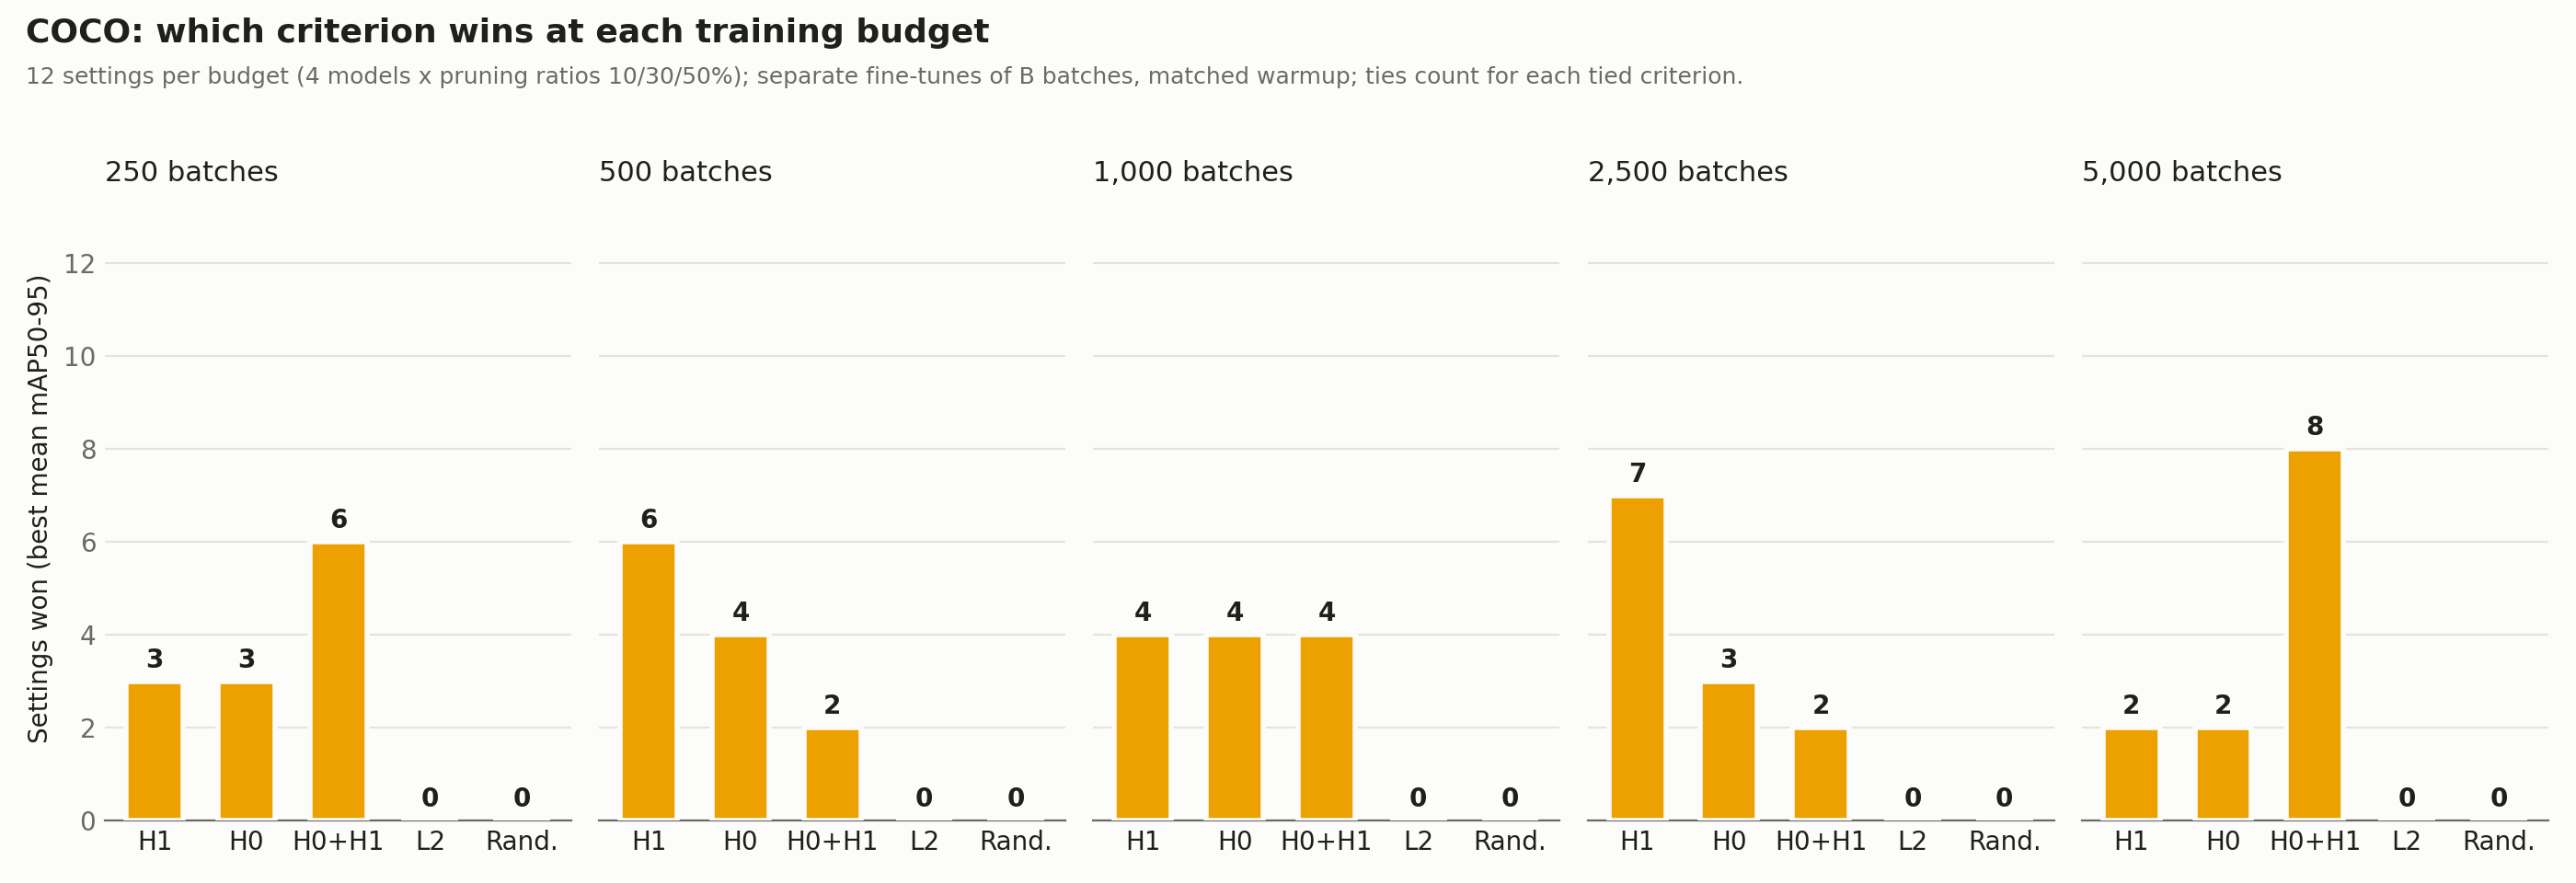
\includegraphics[width=\linewidth]{figures/budget_wins_coco.png}
\tnote{A persistence score wins every COCO setting at every budget; L2 and random never do.
Field~H1 leads at 500 and 2,500 batches, field~H0+H1 at 250 and 5,000.}
\end{figure}

\begin{figure}[H]
\centering
\caption{All datasets: which criterion wins at each training budget}
\label{fig:budgetwins}
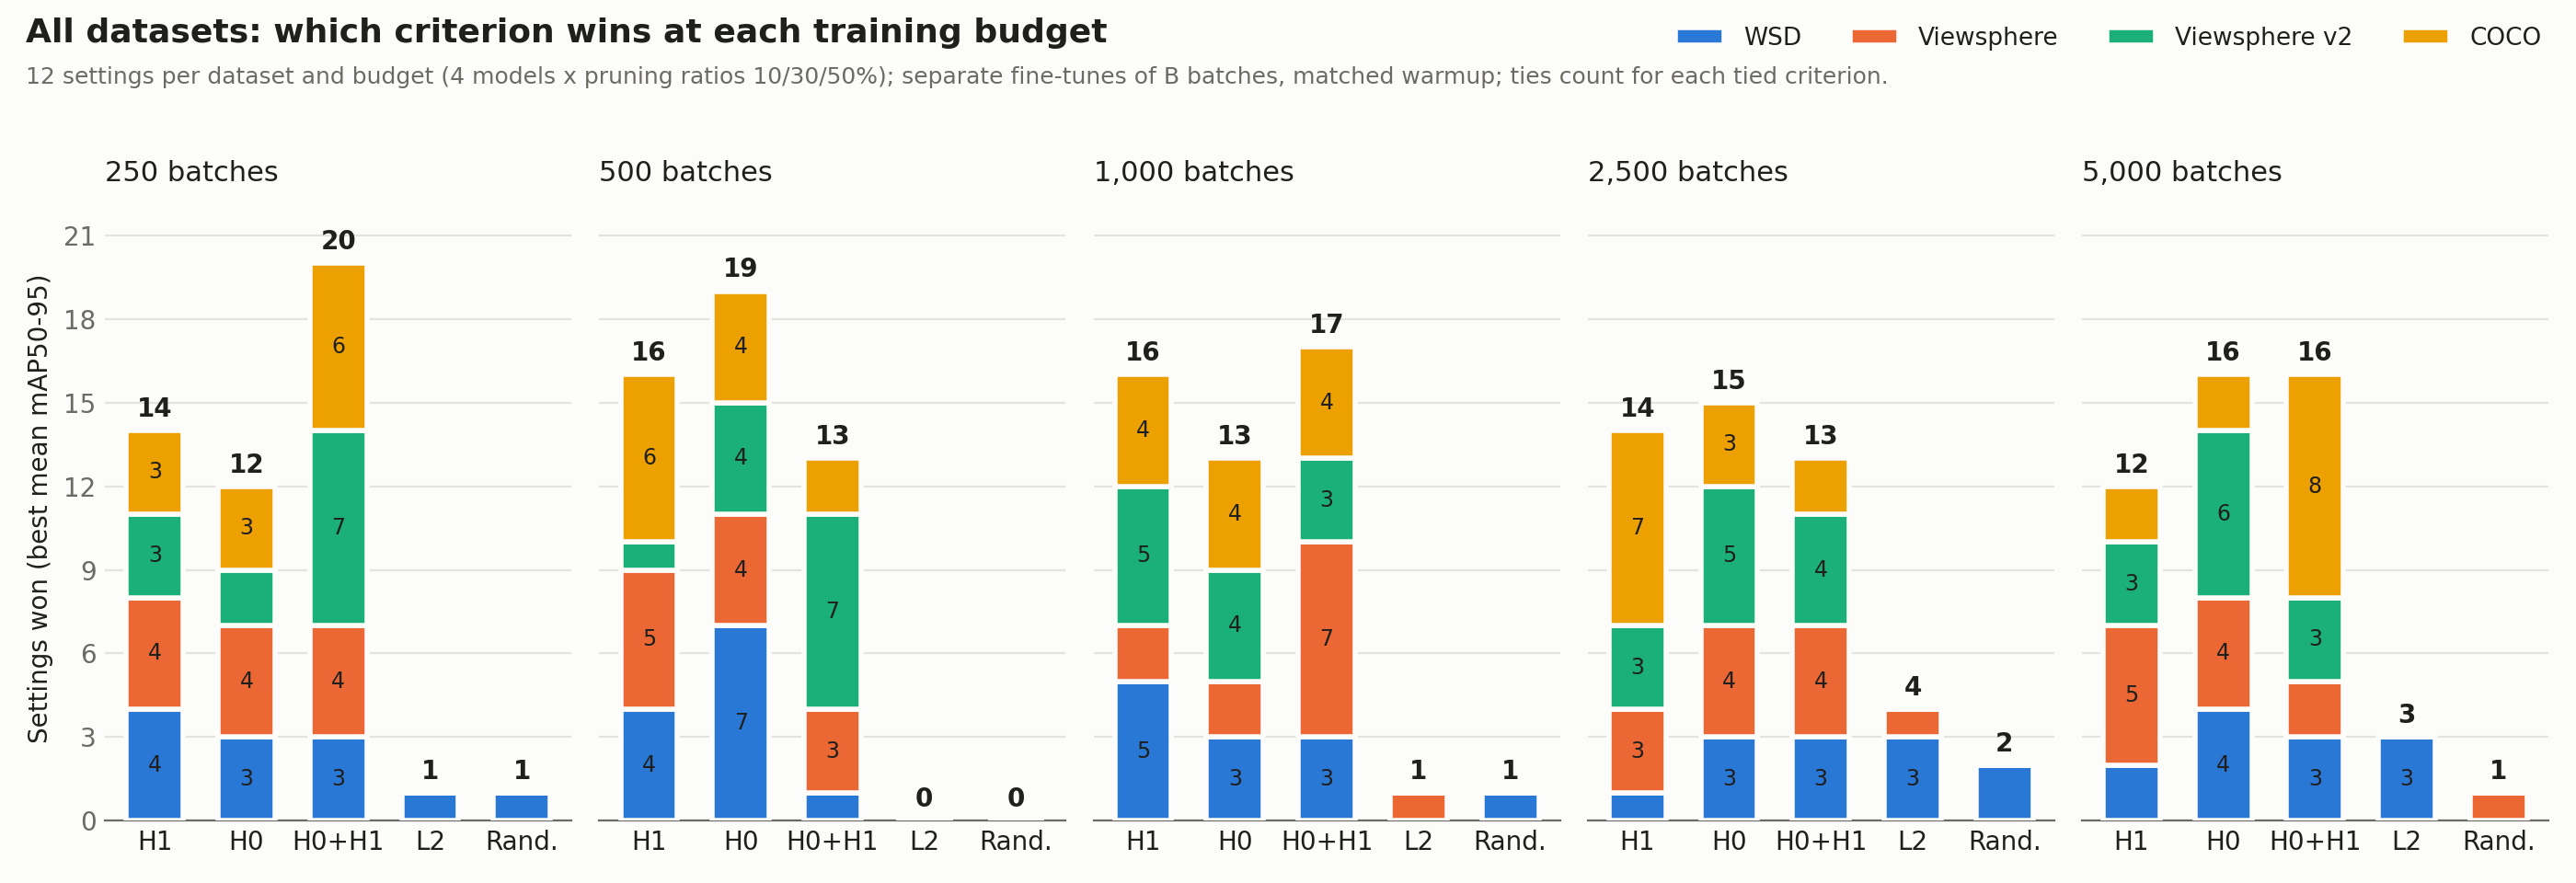
\includegraphics[width=\linewidth]{figures/budget_wins.png}
\tnote{Figures~\ref{fig:bw-wsd}--\ref{fig:budgetwins} stacked. A persistence score wins 42--48 of
the 48 settings at every budget. Which one varies: field~H0+H1 most often at 250 and 1,000 batches,
field~H0 at 500 and 2,500, H0 and H0+H1 tied at 5,000. L2 wins 9 settings in all (7 on WSD), random 5.}
\end{figure}

\subsection{Block replacement, all datasets}

\textbf{Does the block criterion matter?} Table~\ref{tab:blockgap} compares each TDA ranking with
cutting the same number of blocks at random. Random choices already spread (sd up to 0.04
mAP50-95), so \emph{which} blocks are cut matters. On every dataset some ranking beats random choice
by a margin that holds up across seeds, but which one differs: on WSD the null ranking scored on H1
alone (+0.006 to +0.033, every $k$ on both models), on Viewsphere the raw head ranking (+0.015 to
+0.020) and L2 over all blocks (+0.020 to +0.038), on COCO the null ranking (up to +0.118 at $k = 3$
on YOLO26n). Others are clearly worse than random (grid on WSD YOLO26s: $-$0.036 at $k = 3$; null
scored on H0 on Viewsphere: down to $-$0.063), so no single ranking is safe to pick in advance.
Scoring blocks on H0 or H1 alone, instead of the blend, often changes the cut set and with it the
result: H1 alone makes null the most reliable ranking on WSD, H0 alone on COCO YOLO26s. The L2
baseline matches or beats the best TDA ranking on Viewsphere and beats random at $k = 2$ on WSD, so
on these datasets a topological block ranking is not needed to beat random choice.

\begin{table}[H]
\centering\small
\caption{Block pruning: TDA-chosen blocks vs randomly chosen blocks}
\label{tab:blockgap}
\tbl{block_gap}
\tnote{First row of each group: mAP50-95 after cutting $k$ random blocks (23 orders, seed 42) and
fine-tuning 20 epochs. Other rows: each TDA ranking's cut (mean of 3 seeds) minus that random mean.
\textbf{Bold} = the gap exceeds two standard errors, i.e.\ the TDA choice is reliably better (+) or
worse ($-$) than a random one. Scores: C = blend of H0 and H1, H0 = H0 only, H1 = H1 only, L2 = RMS
of the block's convolution weights (not run on COCO); \emph{All, raw} = all blocks on unnormalised
scores (L2 only); -- = not run. Equal entries mean the scores pick the same blocks.}
\end{table}

\begin{table}[H]
\centering\small
\caption{Block pruning: accuracy of each ranking's cut}
\label{tab:blocks}
\tbl{blocks}
\tnote{mAP50-95 after cutting $k$ blocks and fine-tuning 20 epochs. Each ranking's cut is the mean of
3 seeds; the baseline is the spread of 23 random block orders (seed 42); uncut mAP in brackets.
Scores as in Table~\ref{tab:blockgap}. \textbf{Bold} = best ranking and score at that $k$;
$^\dagger$ = above every random order. Rankings that pick the same blocks share one trained model.}
\end{table}

\subsection{Inference cost}

\begin{table}[H]
\centering\small
\caption{Size and inference time of channel-pruned models}
\label{tab:cost}
\tbl{cost}
\tnote{The same for every criterion at a given ratio. GPU: NVIDIA A100, FP16, batch-1 latency (ms)
and batch-32 throughput (images/s); CPU: Intel Xeon, FP32, 8 threads, batch-1 latency (ms). All
three datasets were timed in one run, on the earlier starting models; the pruned shapes depend only
on the ratio, so the timings carry over. \textbf{Bold} = best value for that dataset and model (lowest
GFLOPs and latency, highest throughput).}
\end{table}

Pruning 50\% of channels removes 26--28\% of GFLOPs but changes GPU batch-1 latency by only 1--4\%:
at this model size the GPU is limited by kernel launches, not arithmetic. Batch-32 throughput even
drops at 10--20\% before rising 9--15\% at 50\%. CPU latency improves mainly at 50\% (12--18\%
on WSD and COCO; the Viewsphere CPU timings are noisier). Replacing a block, by contrast, saves
7--14\% GPU latency for one block and 18--28\% for three.

%======================================================================
\section{YOLOv5}
\label{sec:v5}

The whole study was repeated on YOLOv5n/s, in Ultralytics' anchor-free version (YOLOv5u): the
same datasets, criteria, seeds, fine-tunes and recovery budgets as for YOLO26. Starting models:
COCO = Ultralytics' pretrained weights; WSD and Viewsphere = those fine-tuned on each, as for YOLO26
(best mAP50-95 0.409 / 0.434 for n / s on WSD, 0.568 / 0.604 on Viewsphere). YOLOv5 has
no attention layers, so the same channel pruning removes more: at 50\%, 57--61\% of parameters and
35--41\% of GFLOPs (YOLO26: 39\% and 26--28\%). Its replaceable blocks are the eight C3 blocks
(2, 4, 6, 8 in the backbone; 13, 17, 20, 23 in the head). Tables~\ref{tab:wsd5}--\ref{tab:cost5}
match Tables~\ref{tab:wsd}--\ref{tab:cost}.

\subsection{Channel pruning}

\begin{table}[H]
\centering\small
\caption{YOLOv5, WSD: channel pruning by criterion}
\label{tab:wsd5}
\tbl{wsd_channel_v5}
\tnote{As Table~\ref{tab:wsd}.}
\end{table}

\begin{table}[H]
\centering\small
\caption{YOLOv5, Viewsphere: channel pruning by criterion}
\tbl{viewsphere_channel_v5}
\tnote{As Table~\ref{tab:wsd}.}
\end{table}

\begin{table}[H]
\centering\small
\caption{YOLOv5, COCO: channel pruning by criterion}
\tbl{coco_channel_v5}
\tnote{As Table~\ref{tab:wsd}.}
\end{table}

\begin{itemize}
\item \textbf{WSD:} as on YOLO26, the persistence scores are best one-shot at every ratio (n, 10\%:
  0.376--0.380 vs L2 0.350 and random 0.309; s, 50\%: field~H1 0.155 vs L2 0.061). After fine-tuning
  everything is within 0.01 at 10--30\%; at 50\% the persistence scores reach 0.393--0.395 on n (L2
  0.384, random 0.378) and 0.417--0.422 on s (0.407 and 0.415).
\item \textbf{Viewsphere:} one-shot, the persistence scores lead L2 widely (30\%: 0.235--0.245 vs
  0.124 on n, 0.405--0.412 vs 0.221 on s), and L2 is close to random. After fine-tuning they are ahead
  of both at 50\% (0.479--0.482 vs 0.450 and 0.438 on n; 0.535--0.543 vs 0.515 and 0.525 on s); at 10\%
  on s, L2 is best (0.595, holding up).
\item \textbf{COCO:} the persistence scores are best again, but by less than on YOLO26 and with L2
  no better than random: one-shot at 10\%, 0.141--0.148 vs 0.105 (L2) and 0.110 (random) on n;
  after fine-tuning at 50\%, 0.108 vs 0.095 and 0.099 (n) and 0.208--0.212 vs 0.188 and 0.196 (s).
  The three persistence scores give almost the same models after fine-tuning.
\end{itemize}

\subsection{Recovery}

\begin{table}[H]
\centering\small
\caption{YOLOv5: recovery after channel pruning, by training budget}
\tbl{recovery_v5}
\tnote{As Table~\ref{tab:rec}.}
\end{table}

\begin{table}[H]
\centering\small
\caption{YOLOv5, COCO: recovery with longer fine-tunes}
\tbl{recovery_coco_long_v5}
\tnote{As Table~\ref{tab:reclong}.}
\end{table}

\begin{table}[H]
\centering\small
\caption{YOLOv5: training needed to reach 95\% of the unpruned model}
\tbl{recovery_speed_v5}
\tnote{As Table~\ref{tab:speed}.}
\end{table}

On COCO the best persistence score recovers fastest at 50\% at every budget, but the margins are
small (0.001--0.02; after 7 epochs on all of train2017, 0.190--0.192 vs 0.186 on n). YOLOv5 recovers more
slowly than YOLO26 on COCO: even 10\% pruning reaches 95\% of the unpruned model only on s after 3
full epochs (and on n only with field~H1, after 7). On WSD, 50\% pruning is back to 95\% of the
unpruned model within 250 batches on s with every persistence score (L2: 500; random: 1,000), but on n
only with field~H0 (2,500) and H0+H1 (5,000); on Viewsphere 50\% gets there only on s, with field~H1
and H0 after 5,000 batches.

\subsection{Block replacement}

\begin{table}[H]
\centering\small
\caption{YOLOv5 block pruning: TDA-chosen blocks vs randomly chosen blocks}
\tbl{block_gap_v5}
\tnote{As Table~\ref{tab:blockgap}.}
\end{table}

\begin{table}[H]
\centering\small
\caption{YOLOv5 block pruning: accuracy of each ranking's cut}
\tbl{blocks_v5}
\tnote{As Table~\ref{tab:blocks}.}
\end{table}

The pattern by dataset is close to YOLO26's, which suggests it comes from the data rather than the
network. On WSD the null ranking scored on H1 beats random at every $k$ on n (+0.016 to +0.022), and the
head ranking does at $k = 3$ on both models (+0.017). On Viewsphere the raw head ranking beats random at
every $k$ (+0.010 to +0.047) and L2 over all blocks even more at $k = 3$ (+0.049 and +0.063), while grid
and null are mostly worse than random (down to $-$0.083). On COCO most rankings beat random by a
margin that holds up (up to +0.083: null scored on H0 alone, $k = 3$ on n).

\subsection{Inference cost}

\begin{table}[H]
\centering\small
\caption{YOLOv5: size and inference time of channel-pruned models}
\label{tab:cost5}
\IfFileExists{tables/cost_v5.tex}{\tbl{cost_v5}}{\emph{(The YOLOv5 timing run is still in the queue.)}}
\tnote{As Table~\ref{tab:cost}; timed in the same run as the YOLO26 models.}
\end{table}

YOLOv5 runs about a third faster than YOLO26 at batch 1 on the GPU (5.9 vs 9.1~ms unpruned), despite
having more GFLOPs. As on YOLO26, channel pruning barely moves GPU batch-1 latency: removing 35--41\%
of GFLOPs at 50\% leaves it at 5.9~ms, and 10--40\% pruning is slightly slower than none. Batch-32
throughput rises 17--24\% at 50\% and CPU latency falls 18--26\%, more than on YOLO26 because more of
the network is pruned. Replacing blocks saves 5--11\% GPU latency for one block and 15--23\% for three.

%======================================================================
\section{Viewsphere v2}
\label{sec:vs2}

Viewsphere~v2 renders 17 satellites (the 4 of v1 plus AcrimSAT, CALIPSO, CloudSat~B and~C, a 2U
CubeSat, EO-1, GRACE, ICESat-2, Landsat~5 and~8, Jason-2, QuikSCAT and TDRS-D), relabelled to WSD's
4 classes and split by viewing angle exactly as v1 (4,079 / 680 / 680 train / val / test images).
The whole study was run on it for both architectures, with v1's settings (lr $1.25\times10^{-3}$,
matched warmup bias lr; budgets 250--5,000 batches, here 1--20 epochs) but without the
activation-basis grid. Starting models = the COCO models fine-tuned on v2 with pixel noise, best
mAP50-95 0.492 / 0.520 (YOLO26n/s) and 0.477 / 0.518 (YOLOv5n/s), lower than on v1 (0.57--0.63).

\textbf{Black backgrounds and pixel noise.} About 96\% of the pixels in the renders are exactly black
(WSD: 38\%). Models fine-tuned on them without noise became hypersensitive to tiny changes on that
background: noise of $10^{-3}$ on the black pixels moved class scores by up to 0.7--0.96, while the same
noise on the satellite moved them by about 0.01. It showed three ways: fp16 and fp32 inference
disagreed (YOLOv5n: 0.48 vs 0.11 val mAP50-95), validation curves swung from epoch to epoch, and
re-estimating BatchNorm statistics collapsed the \emph{unpruned} model for some calibration seeds
(YOLO26n: 0.09 instead of 0.44), which made the earlier one-shot results on v2 noise. Gaussian pixel
noise during fine-tuning (standard deviation drawn per image from 0 to 3 gray levels), and on the
BatchNorm calibration images, removes all three: fp16 and fp32 agree, BatchNorm re-estimation lands
within 0.004 of the trained model for every seed, and test mAP50-95 drops by only 0.006--0.015. All
Viewsphere runs (v1 and v2) in this report use it.

\subsection{Channel pruning}

\begin{table}[H]
\centering\small
\caption{Viewsphere v2, YOLO26: channel pruning by criterion}
\label{tab:vs2}
\tbl{viewsphere2_channel_vs2}
\tnote{As Table~\ref{tab:wsd}.}
\end{table}

\begin{table}[H]
\centering\small
\caption{Viewsphere v2, YOLOv5: channel pruning by criterion}
\tbl{viewsphere2_channel_v5_vs2}
\tnote{As Table~\ref{tab:vs2}.}
\end{table}

\begin{itemize}
\item \textbf{YOLO26:} one-shot, the persistence scores lead by far, and L2 is worse than random (10\%
  on n: 0.375--0.408 vs L2 0.299 and random 0.331). After fine-tuning, all criteria are within 0.015 at
  10--30\%; at 50\% the persistence scores reach 0.425 on n (L2 0.380, random 0.397) and 0.476--0.482 on
  s (0.455 and 0.467), where field~H1's lead holds up.
\item \textbf{YOLOv5:} the same order, and the single-seed collapses of the earlier models are gone
  (every seed at 50\% within 0.01 of the others). At 50\%: 0.403--0.407 vs 0.343 (L2) and 0.372 (random)
  on n, 0.449--0.453 vs 0.401 and 0.434 on s. One-shot at 10\%, L2 is again below random (0.283 and
  0.293 vs 0.334 and 0.413).
\end{itemize}

\subsection{Recovery}

\begin{table}[H]
\centering\small
\caption{Viewsphere v2, YOLO26: recovery after channel pruning, by training budget}
\tbl{recovery_vs2}
\tnote{As Table~\ref{tab:rec}.}
\end{table}

\begin{table}[H]
\centering\small
\caption{Viewsphere v2, YOLOv5: recovery after channel pruning, by training budget}
\tbl{recovery_v5_vs2}
\tnote{As Table~\ref{tab:rec}.}
\end{table}

\begin{table}[H]
\centering\small
\caption{Viewsphere v2, YOLO26: training needed to reach 95\% of the unpruned model}
\tbl{recovery_speed_vs2}
\tnote{As Table~\ref{tab:speed}; the budgets are 1--20 epochs here.}
\end{table}

\begin{table}[H]
\centering\small
\caption{Viewsphere v2, YOLOv5: training needed to reach 95\% of the unpruned model}
\tbl{recovery_speed_v5_vs2}
\tnote{As Table~\ref{tab:speed}.}
\end{table}

With the noise fix the unpruned models improve steadily with budget (YOLO26n: 0.464 after 250
batches, 0.488 after 5,000), so batches-to-95\% tables are meaningful here too. At 50\%, the
persistence scores lead L2 and random at every budget, most of all early (YOLO26n, 1,000 batches:
0.335--0.360 vs 0.224 and 0.260) and still at 5,000 (0.424--0.425 vs 0.379 and 0.397; unpruned 0.488).
Light pruning (10\%) reaches 95\% of the unpruned model within 250--1,000 batches with the persistence
scores, but needs 1,000--2,500 with L2; 50\% never gets there within 5,000 batches (20 epochs).

\subsection{Block replacement}

\begin{table}[H]
\centering\small
\caption{Viewsphere v2 block pruning: TDA-chosen blocks vs randomly chosen blocks, YOLO26}
\tbl{block_gap_vs2}
\tnote{As Table~\ref{tab:blockgap}.}
\end{table}

\begin{table}[H]
\centering\small
\caption{Viewsphere v2 block pruning: TDA-chosen blocks vs randomly chosen blocks, YOLOv5}
\tbl{block_gap_v5_vs2}
\tnote{As Table~\ref{tab:blockgap}.}
\end{table}

\begin{table}[H]
\centering\small
\caption{Viewsphere v2 block pruning: accuracy of each ranking's cut, YOLO26}
\tbl{blocks_vs2}
\tnote{As Table~\ref{tab:blocks}.}
\end{table}

\begin{table}[H]
\centering\small
\caption{Viewsphere v2 block pruning: accuracy of each ranking's cut, YOLOv5}
\tbl{blocks_v5_vs2}
\tnote{As Table~\ref{tab:blocks}.}
\end{table}

On YOLO26 the gaps to random choice are small (within $\pm$0.017, and the random cuts themselves
spread only 0.005--0.016): the largest that hold up are L2 over all blocks on s (+0.014 and +0.010 at
$k = 2, 3$) and the null ranking scored on H1 at $k = 3$ on n (+0.010). On YOLOv5 the picture is v1's:
the raw head ranking beats random at every $k$ (+0.006 to +0.015, except H1 at $k = 2$ on s), L2 over
all blocks does too, by most at $k = 3$ (+0.028 and +0.030), and grid is worse than random everywhere
(down to $-$0.056), null mostly.

\end{document}
